\chapter{Estado del arte}\label{sec:Estado_arte}
En la presente sección se desarrollarán los aspectos teóricos a tener en cuenta para un correcto entendimiento del trabajo realizado. Además se presentará la evolución de algunos sistemas, así como sus ventajas e inconvenientes.
\section{Concepto FPGAs}
Una FPGA o (Field programmable Gate Arrays) es un dispositivo reconfigurable que puede ser eléctricamente programado para implementar una alta variedad de circuitos lógicos. Consiste en un "array" uniforme de estructuras lógicas programables que son interconectadas por una configurable red de enrutamiento. Un ejemplo de una red de enrutamiento puede verse en la figura \ref{fig:estructura_FPGA}

\begin{center}
	\begin{figure}[H]
		\center
		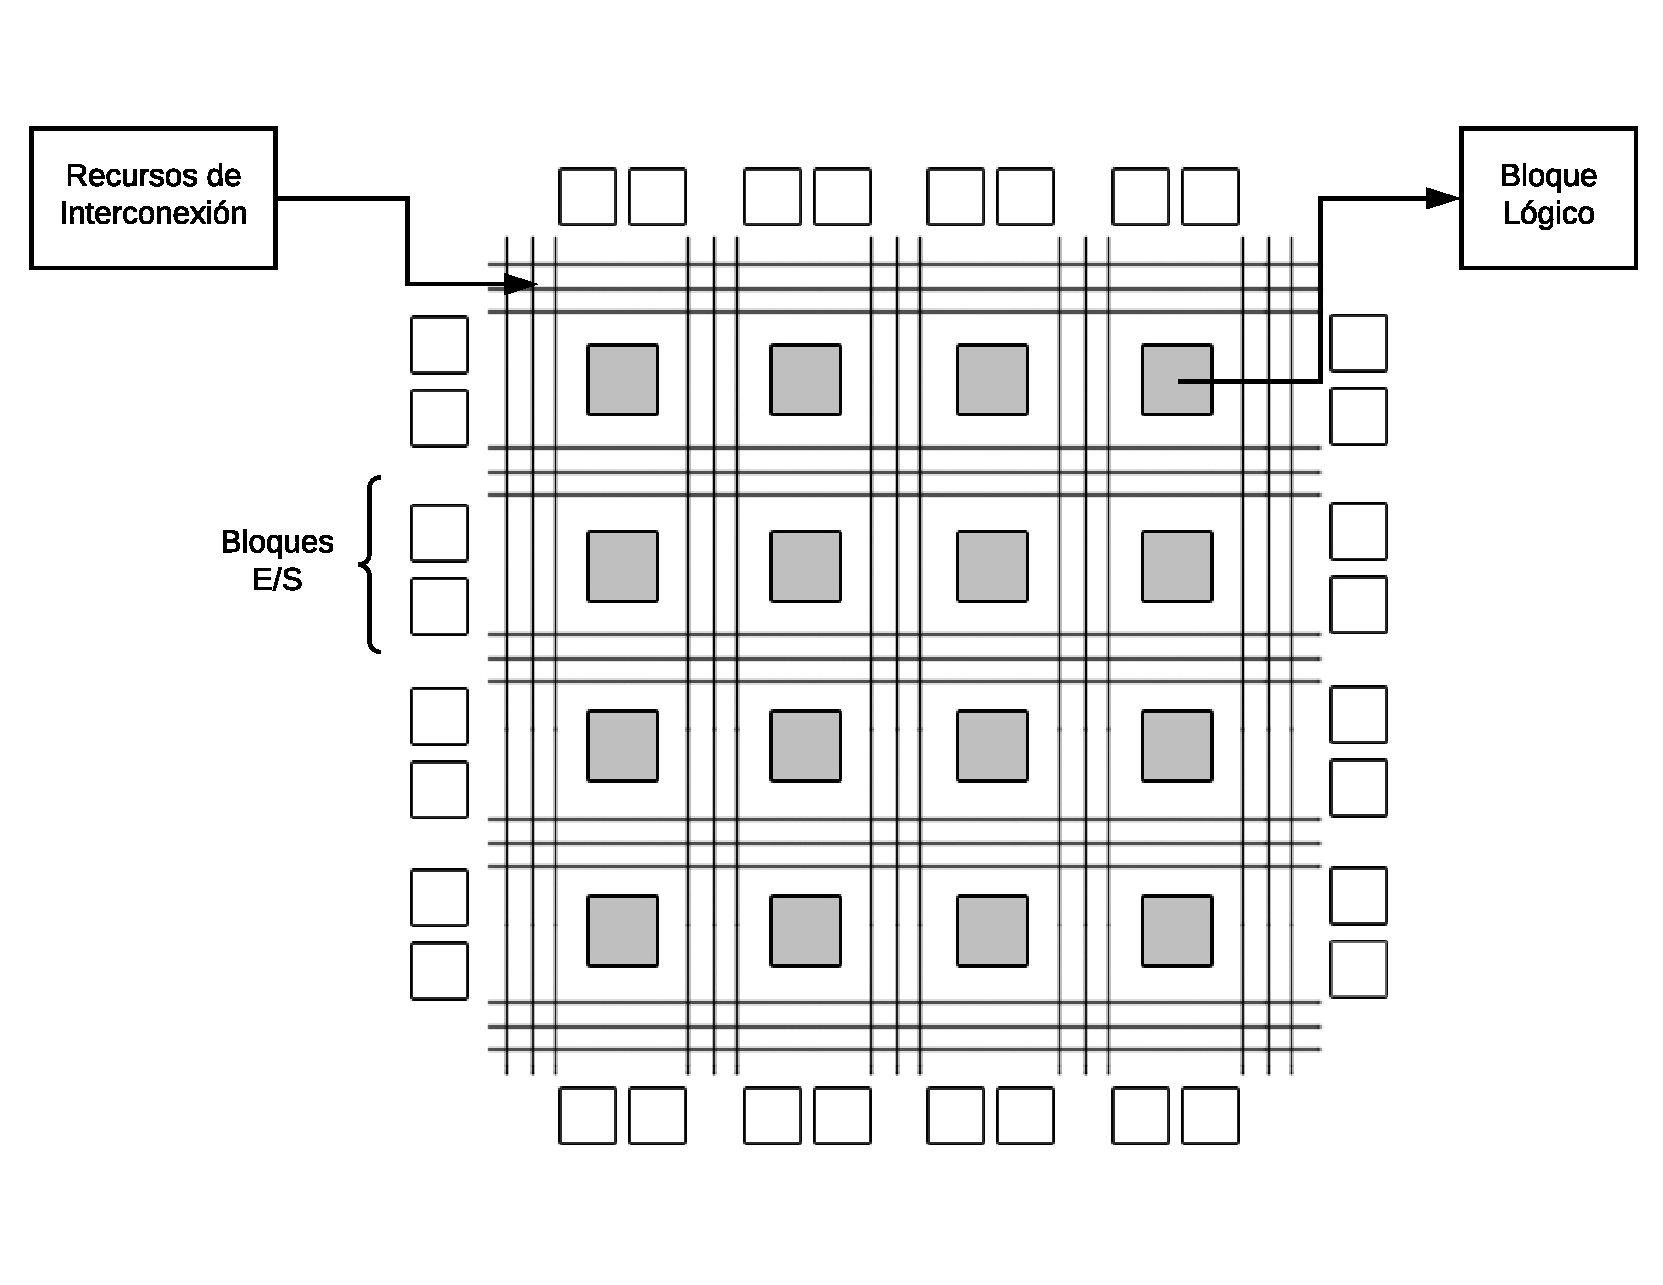
\includegraphics[trim = 0mm 10mm 0mm 10mm, clip,scale=0.4]{imagenes/EstadoArte/estructura_FPGA.pdf}
		\caption{PLD vs FPGA}
		\label{fig:estructura_FPGA}
	\end{figure}
\end{center}
 Lo lógica y las estructuras de interconexión pueden ser configuradas gracias a potentes herramientas CAD, las cuáles permiten que el usuario final pueda definir esta interconexión física de bloques lógicos mediante lenguajes de descripción hardware (Hardware Description Languaje, HDL). Algunos de los más conocidos son VHDL, Verilog o ABEL. 
\newline
Si bien no es el más usado actualmente, a lo largo de la sección \ref{sec:Verilog} se realizará una breve introducción a Verilog, comentando y analizando sus principales características.
\newpage
\subsection{Evolución y escenario}

Las FPGAs fueron inventadas en el año 1984 por Ross Freeman y Bernard Vonderschmitt, co-fundadores de Xilinx. Originalmente fueron diseñadas para servir como prototipos o demostraciones de la funcionalidad de circuitos digitales. Las FPGAs conforman la máxima evolución de los PLDs (Programmable Logic Device), definidos estos como circuitos integrados en los que se pueden programar ecuaciones lógicas booleanas. Algunos de sus usos en la actualidad son: 
\begin{itemize}
	\item Sistemas de visión artificial.
	\item Sistemas de imágenes médicas.
	\item Codificación y encriptación.
	\item Reconocimiento de voz.
	\item Aeronáutica y defensa.
\end{itemize}
\newline

El revolucionario éxito de estos dispositivos programables puede ser atribuido a la flexibilidad en la implementación del diseño. Así, la capacidad de re-programar al instante la FPGA con varios circuitos sin costo adicional, promueve la re-utilización del dispositivo, permite una rápida verificación del diseño y por ello, reduce el gasto en la etapa de desarrollo. Si bien actualmente no representan todo el sistema de un producto final, sus ventajas en las propiedades del diseño hacen que estén empezando a formar parte de una pieza importante en el desarrollo de un producto electrónico. \newline

Para intentar entender el porqué de la importancia de dispositivos de implementación hardware sería adecuado introducir la Ley de Moore. La ley de Moore expresa que aproximadamente cada dos años se duplica el número de transistores en un microprocesador. Como se puede ver en la figura \ref{fig:Ley_de_Moore}, esta ley que formuló el cofundador de Intel E. Moore el 19 de Abril de 1965 no se aleja de la realidad: 
\newline
\begin{figure}[H]
	\center
	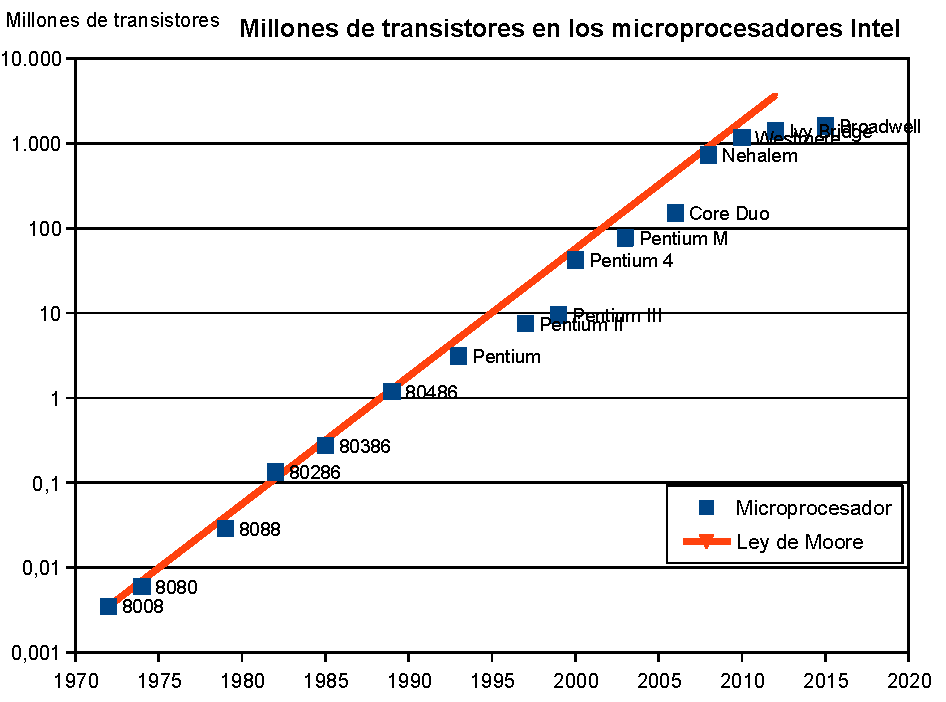
\includegraphics[scale=0.7]{imagenes/EstadoArte/ley_moore-eps-converted-to.pdf}
	\caption{Ley de Moore}
	\label{fig:Ley_de_Moore}
\end{figure}
 

No obstante, tal y como ya han anunciado las principales empresas de microprocesadores actuales como son Intel y AMD en su hoja de ruta tecnológica para semiconductores, la ley de Moore llegará a su fin en 2021. Después de esa fecha, no resultará económicamente eficiente reducir más el tamaño de los transistores de silicio. La predicción de la industria no es que simplemente su tasa de reducción será cada vez más lenta, sino que se va a detener definitivamente. Es aquí donde la electrónica digital comenzará a tener un papel importante en los microprocesadores. Tanto es así que multinacionales dedicadas a la fabricación de procesadores como pueden ser Intel o AMD ya están trabajando en implementar esos comportamientos en FPGAs. Sus ventajas e inconvenientes serán presentadas en el las secciones \ref{sec:ArquitecturaFPGA} y \ref{sec:DescripcionHardware}.

\subsection{Arquitectura FPGA}\label{sec:ArquitecturaFPGA}

En un PLD, las interconexiones entre elementos ya esta prefijada, y solo es posible habilitar o deshabilitar esta conexión. Por el contrario, sobre FPGA estas interconexiones no están prefijadas, siendo el usuario final el que decide las interconexiones entre bloques lógicos (figura \ref{fig:pld_fpga}).
\newline
\begin{center}
\begin{figure}[H]
	\center
	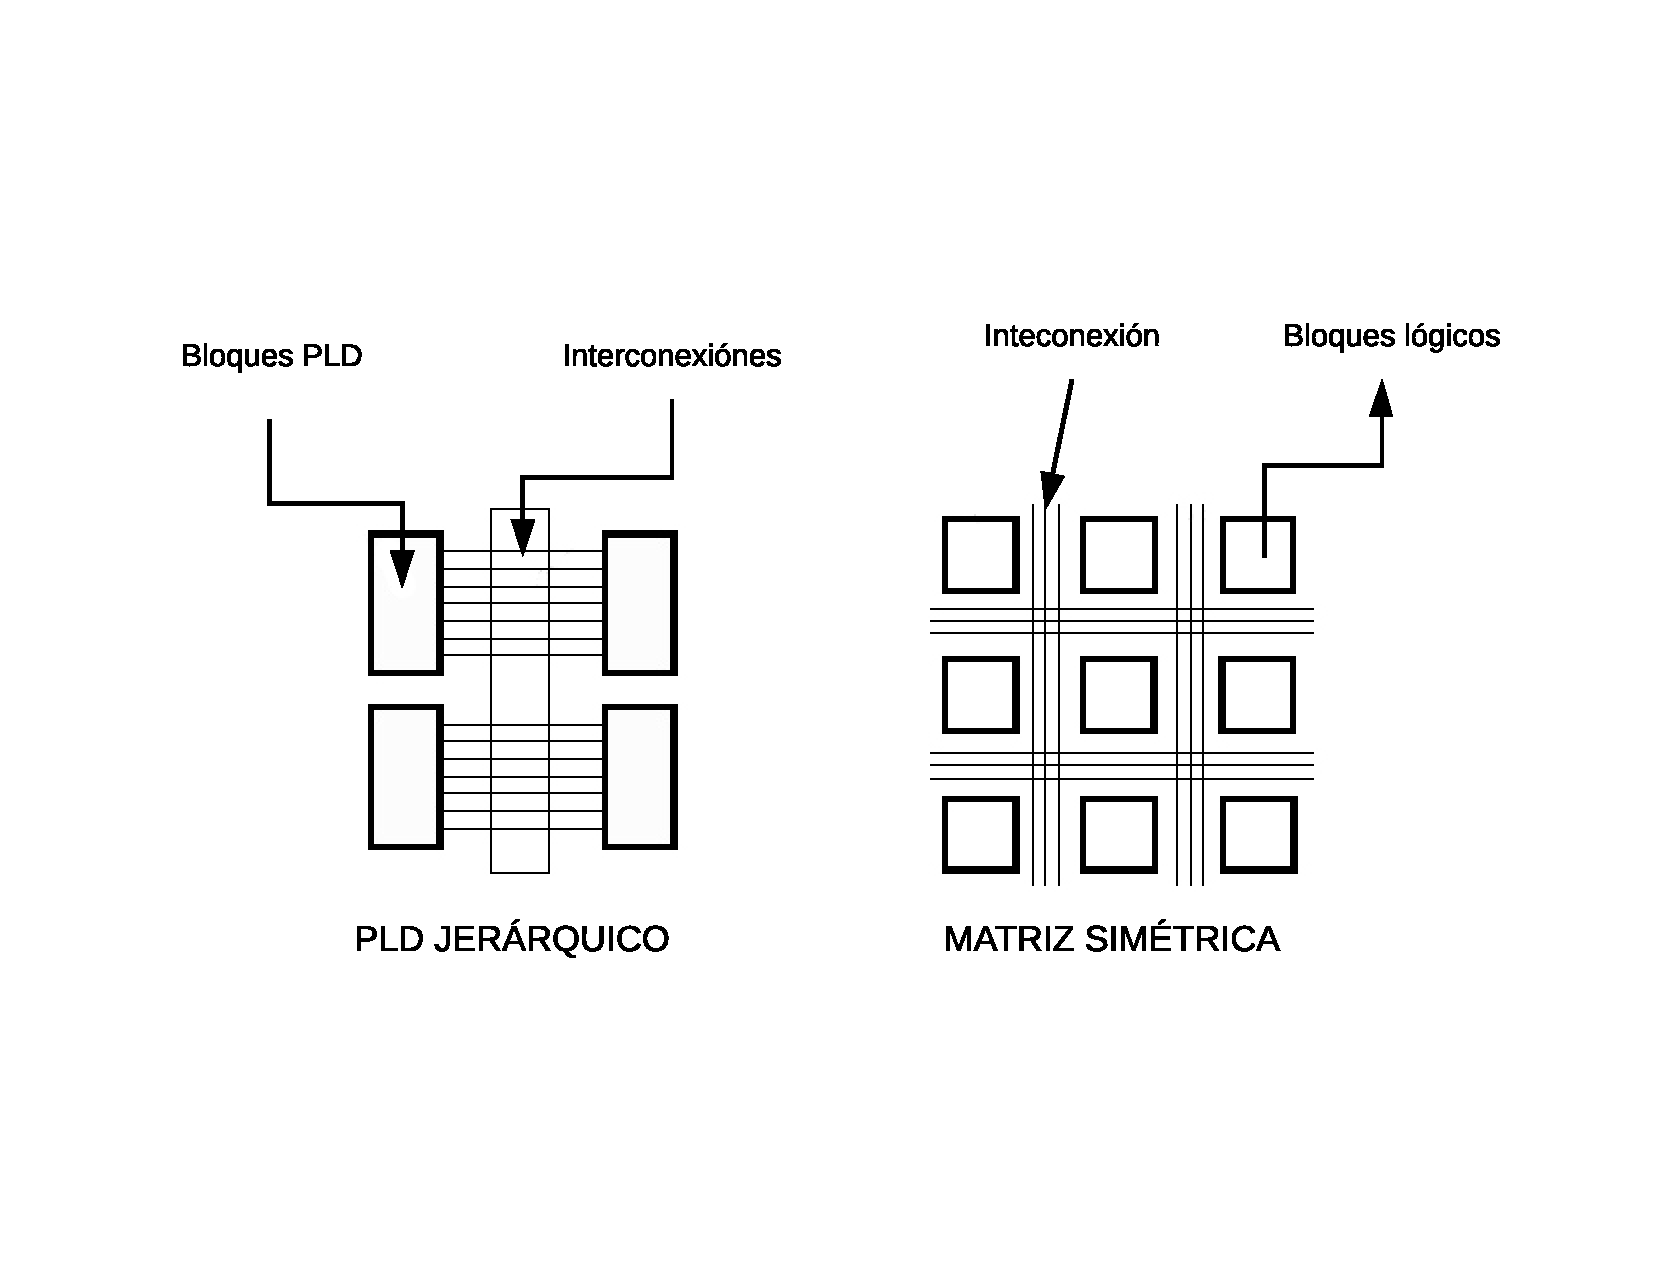
\includegraphics[trim = 10mm 35mm 10mm 35mm, clip,scale=0.6]{imagenes/EstadoArte/pld_fpga.pdf}
	\caption{PLD vs FPGA}
	\label{fig:pld_fpga}
\end{figure}

\end{center}

A la hora de elegir una FPGA para un proyecto determinado es importante tener en cuenta una de sus propiedades más importantes, el número de bloques lógicos. El número de bloques lógicos determinan la capacidad del dispositivo y forma parte de una de las características mas limitantes de las FPGAS en la actualidad. Los bloques lógicos son independientes entre sí y pueden interconectarse para formar un módulo más complejos. \newline

A continuación se introducirán los conceptos de granularidad fina y granularidad gruesa, que dará lugar al correcto entendimiento de la arquitectura en una FPGA. 

Estos módulos más complejos realizan las operaciones básicas que en conjunto representan la función que operará en una FPGA. Se dice que las FPGAs son dispositivos con una arquitectura avanzada por la densidad de sus componentes y por los diferentes caminos de interconexión entre módulos. Así, de acuerdo al tipo de módulos lógicos que la conforman, encontramos dos derivaciones estructurales: 
\begin{itemize}
	\item Granularidad Gruesa.
	\item Granularidad Fina.
\end{itemize}

Los módulos lógicos en una arquitectura de granularidad gruesa son módulos grandes generalmente consistentes de una o más tablas de consulta y dos o más flip-flops. La tabla de consulta, también conocida como LookUp Table (LUT), actúa como una memoria donde se encuentra almacenada la tabla de verdad que representa la función lógica del circuito, así, en una LUT se puede implementar cualquier función deseable. Dependiendo el tamaño de la LookUp Table, se pueden implementar funciones de más o menos variables. \newline

Por otra parte, una arquitectura de granularidad fina, está estructurada por una gran cantidad de módulos lógicos pequeños que realizan funciones relativamente simples. Cada módulo está compuesto de un circuito de dos entradas que realiza una función lógica determinada, o en algunos otros casos por un multiplexor. También suele contener algún flip-flop.  \newline

La FPGAs mas utilizadas actualmente suelen contar con tecnología de granularidad gruesa, que permite elevar el nivel de abstracción con respecto a las FPGA de granularidad fina. \newline

El primer caso permite implementaciones menos detalladas ya que desde un nivel muy básico se tienen módulos más complejos y el hecho de utilizar LUT deja entrever que se pueden realizar diseños más grandes. A lo largo de este proyecto se trabajará con el primer caso, ejemplo de ello es la FPGA utilizada, IceZum Alhambra II. \newline

El diseñador propone la función lógica a realizar a través de métodos de descripción hardware y define los parámetros de su diseño. Esto se hace por medio de código programable, que puede ser un lenguaje de descripción hardware, el cuál es introducido en la sección \ref{sec:DescripcionHardware}. 

\subsection{Lenguajes de descripción hardware}\label{sec:DescripcionHardware}

Un lenguaje de descripción hardware (Hardware Description Languaje, HDL) es un lenguaje usado para modelar el funcionamiento de un bloque hardware en una forma textual. Al igual que podemos encontrar diferencias entre los diferentes tipos de lenguajes de programación en cuanto a su sintaxis de codificación y sus métodos de simulación y síntesis, se observan ciertas diferencias entre HDL's. \newline
Se tienen dos tipos diferentes de lenguajes de descripción hardware:
\begin{itemize}
	\item Bajo modelado. No permiten la jerarquezación de módulos y son capaces de realizar solo descripciones simples.
	\item Alto modelado. Son los mas utilizados actualmente, permiten diseñar sistemas más complejos. Ejemplos de alto modelado son Verilog (Verify Logic) y VHDL (VHSIC Hardware Description Language).
\end{itemize}	
Este trabajo se basará en Verilog por permitir un nivel más alto de implementación que VHDL, como será analizado en la sección \ref{sec:Verilog} . \newline

Ambos lenguajes comparten algunas características comunes, como el soporte para cualquier nivel de modelado y abstracción, y que cada elemento de diseño tiene una interfaz bien definida, para permitir la conexión rápida con otros elementos lógicos.

\subsection{Verilog}\label{sec:Verilog}
Debido a su utilización a lo largo de este proyecto, se analizarán algunas características importantes cuyo conocimiento será básico para entender el código.

\subsubsection{Tipos de datos}

Existen dos tipos de datos en Verilog los cuáles tienen que ser entendidos para poder alcanzar la funcionalidad buscada:
\begin{itemize}
	\item reg: Representan variables con capacidad para almacenar información.
	\item wire: Representan conexiones entre componentes, no tienen capacidad de almacenamiento.
\end{itemize}

\subsubsection{Implementación en módulos}
En la mayoría de los casos y para no perder el nivel de abstracción, un proyecto en Verilog suele estar compuesto por un conjunto de módulos los cuáles forman una funcionalidad completa, y cada uno de ellos, una especifica. \newline

Las características principales de la implementación digital por módulos son:
\begin{itemize}
	\item Cada módulo dispone de una serie de entradas y salidas cuya función principal es interconectar otros módulos, aunque puede no tener entradas y salidas.
	\item No existen variables globales.
	\item Cada módulo puede describirse de forma arquitectural o de comportamiento.
\end{itemize}

Esta implementación por módulos Verilog permite la configuración del nivel de abstracción deseado por el usuario final. El desarrollo de módulos de funcionalidad específica puede tener sus ventajas e inconvenientes dependiendo de su uso final. Si se quieren reutilizar para otros flujos de trabajo (ejemplo: sumador 8 bits), es bueno tener módulos muy definidos según su funcionalidad (ejemplo: sumador de 2 bits). Sin embargo, la polarización no tiene porque ser imprescindible, si bien aconsejada.

\subsubsection{Paralelización de Procesos}
Una de las características mas importantes que diferencia a Verilog del resto de lenguajes procedurales \footnote{lenguajes procedurales: ejecución de la aplicación se inicia con la primera línea de código, y sigue una ruta predefinida a través de la aplicación, llamando procedimientos según sea necesario.} es la posibilidad de ejecutar varios procesos en paralelo, aspecto fundamental en el lenguaje, y el cuál le brinda gran parte de las ventajas de usar implementación hardware.

\begin{center}
	\begin{figure}[H]
		\center
		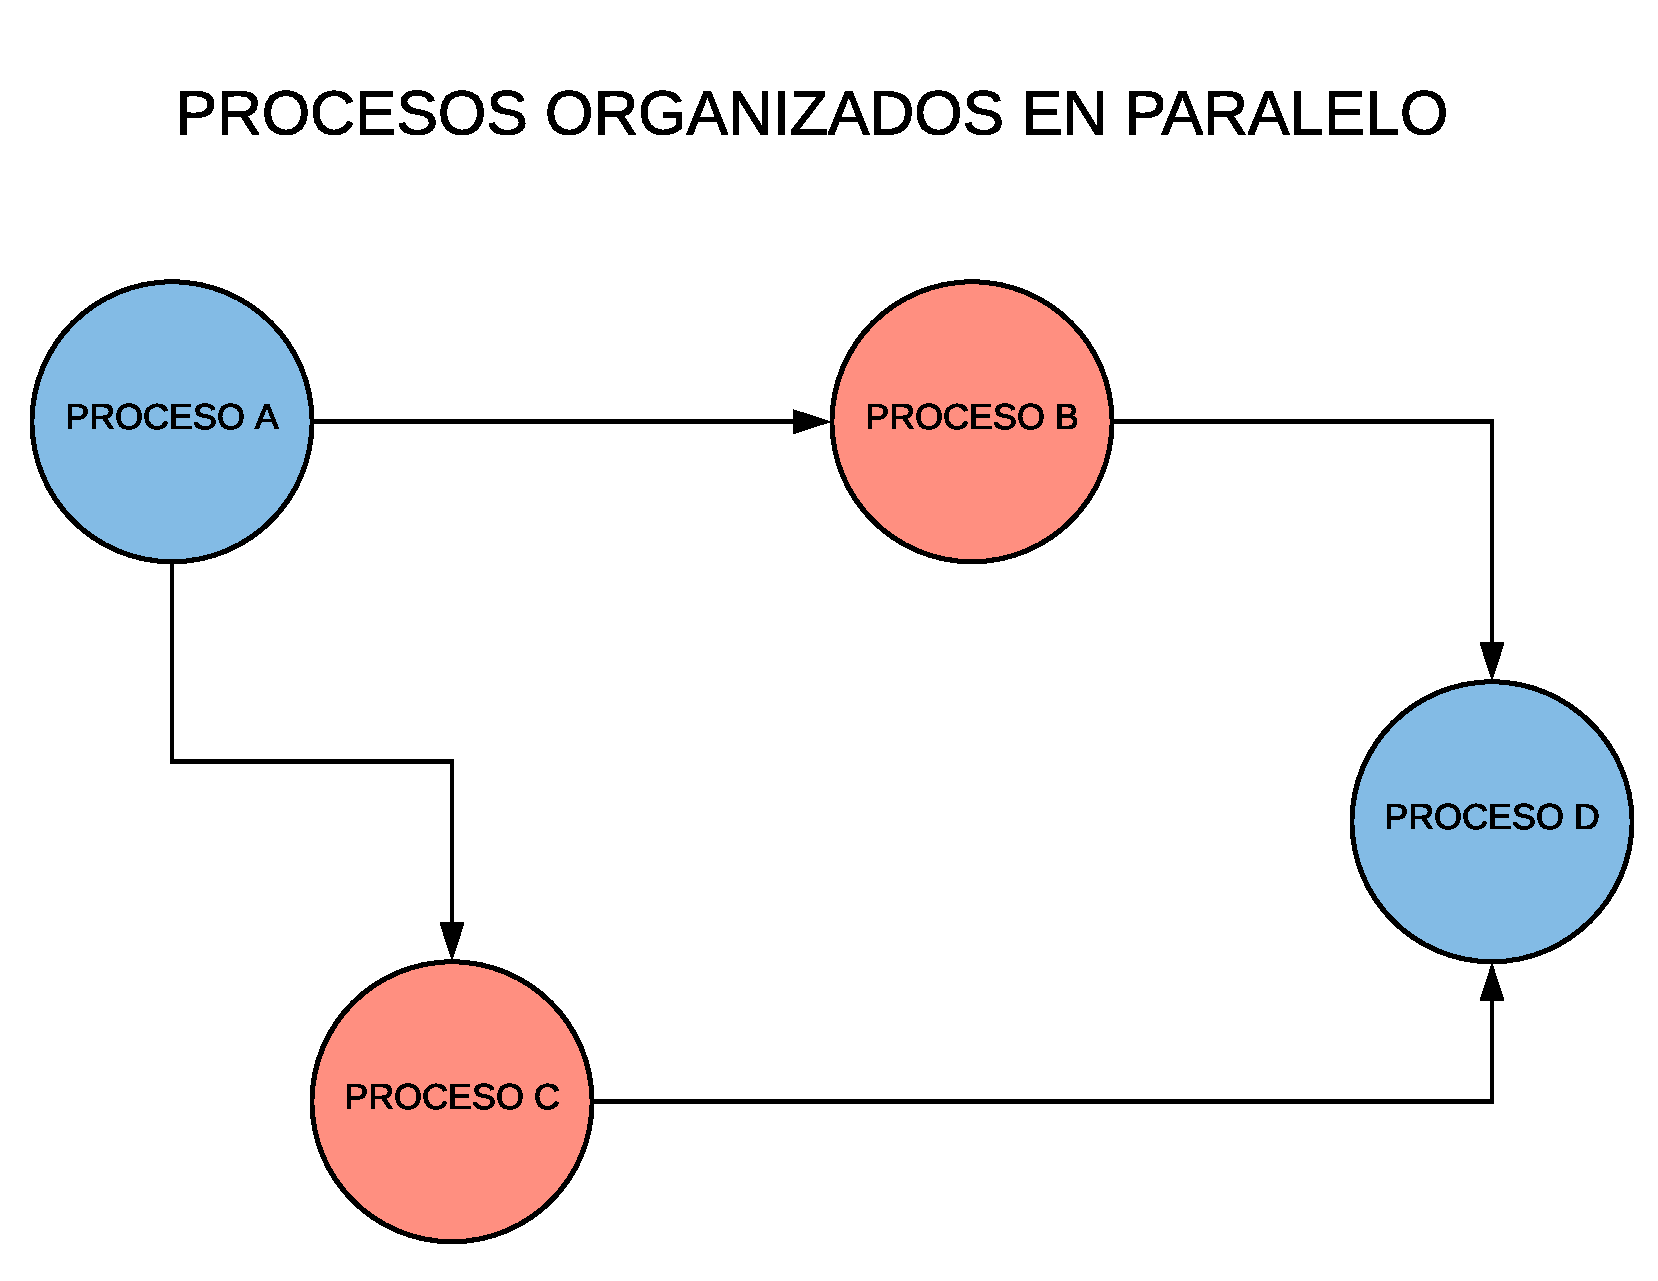
\includegraphics[trim = 0mm 0mm 0mm 0mm, clip,scale=0.3]{imagenes/EstadoArte/procesos_paralelo.pdf}
		\caption{Paralelización de Procesos}
		\label{fig:procesos_paralelo}
	\end{figure}
	
\end{center}
Toda implementación de Verilog se declara dentro de un proceso que puede ser de dos tipos:

\begin{itemize}
		\item Initial: Este tipo de procesos se ejecutan sólo una vez comenzando su ejecución al inicio, y por tanto no existen retardos. Este proceso no es sintetizable, es decir, no puede ser utilizado en una descripción RTL.
		
		\item Always: Este tipo de procesos se ejecuta continuamente a modo de bucle, y como su propio nombre indica, está continuamente ejecutándose. Este proceso si que es sintetizable y es controlado por la temporización o por eventos. Si dicho bloque se ejecuta por más de un evento, dicho conjunto se denomina lista sensible.
\end{itemize}

\subsubsection{Estructuras de control}

Al igual que los leguajes de tipo procedural, Verilog dispone de una serie de estructuras de control:

\begin{itemize}
	\item if - else
	\item Case. Es una de las estructuras de control mas utilizadas a lo largo de este proyecto, permite la generación de máquinas de estados
	\item For
	\item While
	\item Forever
	\item Wait
	
\end{itemize}

\subsubsection{Asignación continua}

Mediante la asignación continua se puede modelar lógica combinacional, es decir, no se necesita una lista de sensibilidad para realizar la asignación. Sólo puede ser declarada fuera de cualquier proceso.

\subsubsection{Asignación procedural}

A las variables se le asigna un valor dentro de un proceso always o initial, el tipo de variable a la que se le asigna el valor puede ser de cualquier tipo.

%%%%%%%%%%%%%%%%%%%%%%%%%%%%%%%%%%%%%%%%%%%%%%%%%%

\section{FPGAs libres}
\subsection{Evolución}
Muchos lenguajes de implementación hardware así como su arquitectura de FPGA utilizada están ligados a importantes empresas tales como Xilinx, Intel (anteriormente Altera), etc, y poder trabajar con ellos requiere un elevado presupuesto. \newline
Lo anterior por lo tanto, lleva a que no muchas empresas ni particulares puedan beneficiarse de las ventajas de la utilización de FPGAs y a su vez, que el avance tecnológico sea aún más lento. Una de las claves del éxito de empresas como Arduino no es más que la comunidad de gente que existe detrás creando nuevas librerías, componentes, etc. Todo ello a su vez gracias al bajo precio de sus productos, y a la posibilidad de encontrar todo el hardware y software en la web. \newline

Para entender el nacimiento de las FPGAs libres es importante conocer qué es el bytestream. \newline
Un bytestream es una secuencia de bytes que se utiliza en telecomunicaciones y computación. El término bystream se utiliza para describir la configuración con la que se implementará un determinado diseño en una FPGA. Este formato detallado de flujo de bits para una FPGA particular es típicamente propietario del proveedor de FPGA. \newline

Es por ello que Clifford Wolf decidió interpretar el bytestream del modelo Lattice iCE40 y desarrolló la herramienta IceStorm. \newline
IceStorm se desarrolló como software de traducción de Verilog (lenguaje de descripción en FPGAs, sección \ref{sec:Verilog}) al bytestream. Esta traducción fue posible gracias a la ingeniería inversa, esto es, no se le da el uso habitual, sino el inverso. 

Ya no se depende de ningun fabricante y todo el conocimiento además esta disponible. A partir de estas herramientas se puede crear cualquier interfaz o cualquier aplicación que no haya sido prevista por el fabricante. \newline

Sólo las FPGAs de Lattice iCE40 (modelos HX1K-TQ144 y HX8K-CT256) son hasta el momento con las que se pueden trabajar (figura \ref{fig:lattice}), pero al ser un proyecto libre \footnote{Proyecto libre: El término libre se refiere a la libertad de los usuarios para ejecutar, copiar, distribuir, estudiar, cambiar y mejorar ese hardware o software.}, muchas personas ya están aumentando sus posibilidades.
\begin{center}
	\begin{figure}[H]
		\center
		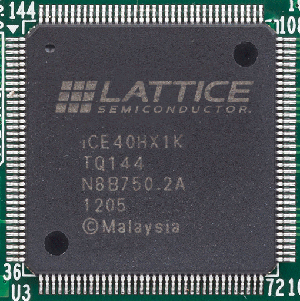
\includegraphics[trim = 0mm 0mm 0mm 0mm, clip,scale=0.5]{imagenes/EstadoArte/lattice.png}
		\caption{Lattice iCE40HX1K}
		\label{fig:lattice}
	\end{figure}
\end{center}

Algunos ejemplos de FPGAs ya disponibles para ser usadas se exponen en las figuras \ref{fig:tiny_fpga}, \ref{fig:blackIceII}, \ref{fig:icoBoard}
\begin{center}
	\begin{figure}[H]
		\center
		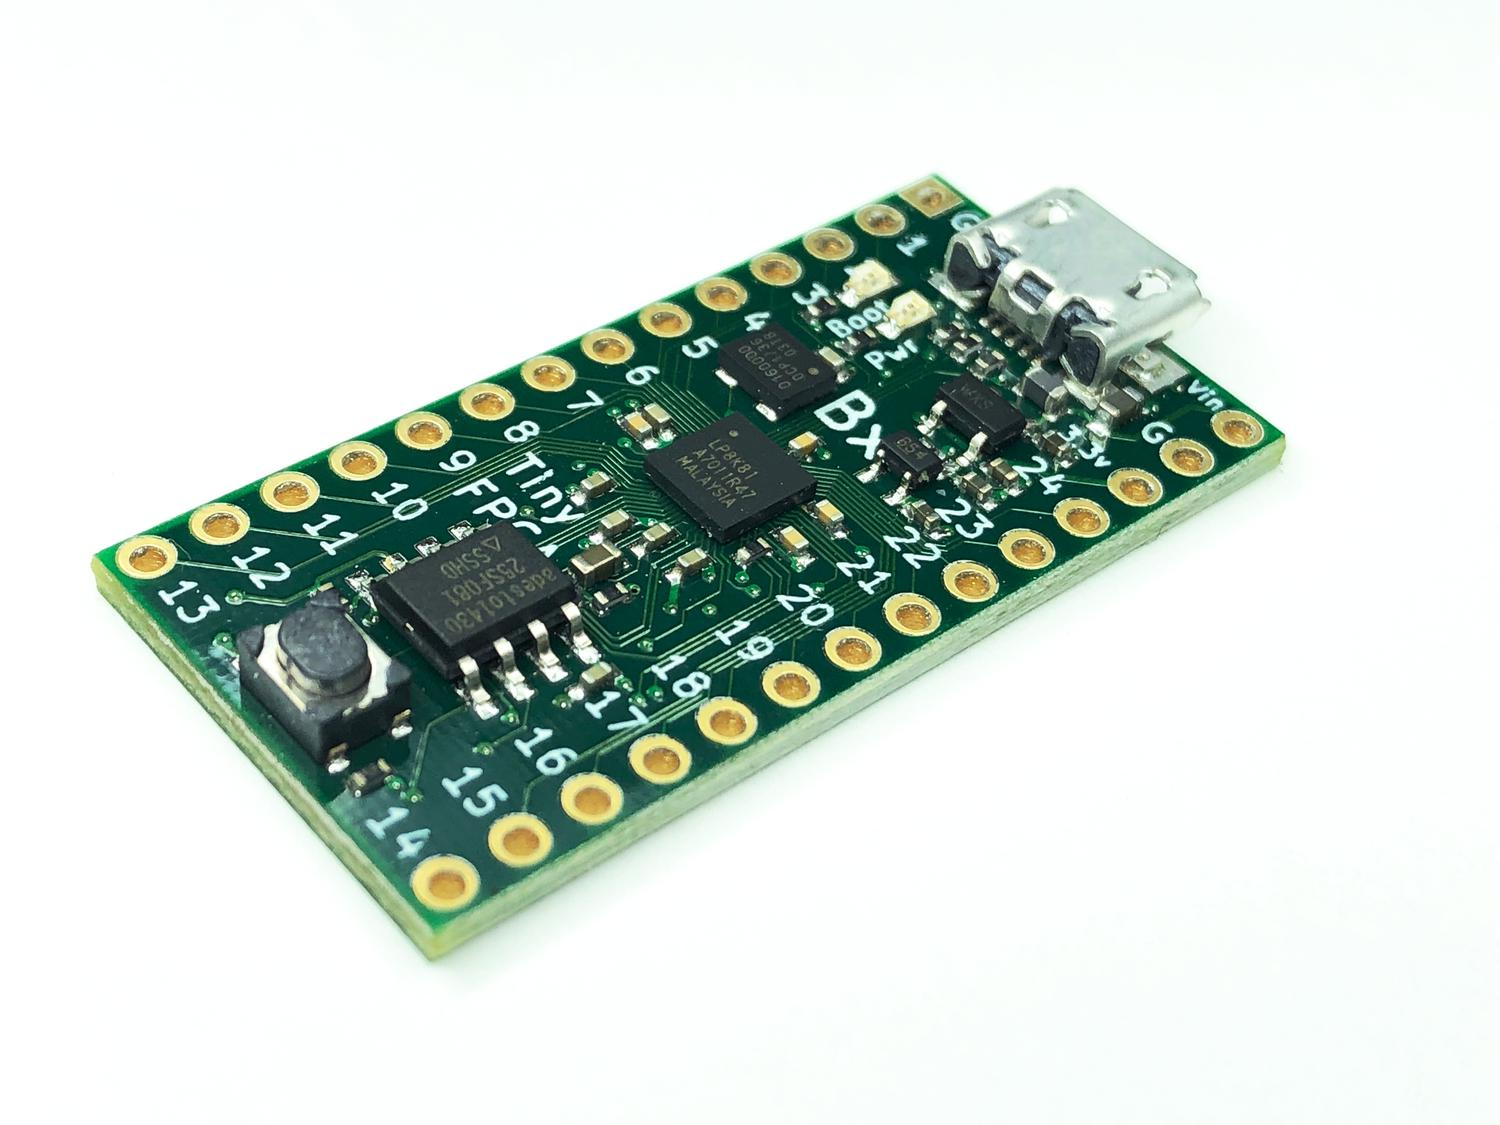
\includegraphics[trim = 0mm 0mm 0mm 0mm, clip,scale=0.2]{imagenes/EstadoArte/tinyFPGABX.jpg}
		\caption{Tiny FPGA BX}
		\label{fig:tiny_fpga}
	\end{figure}
\end{center}
\begin{center}
	\begin{figure}[H]
		\center
		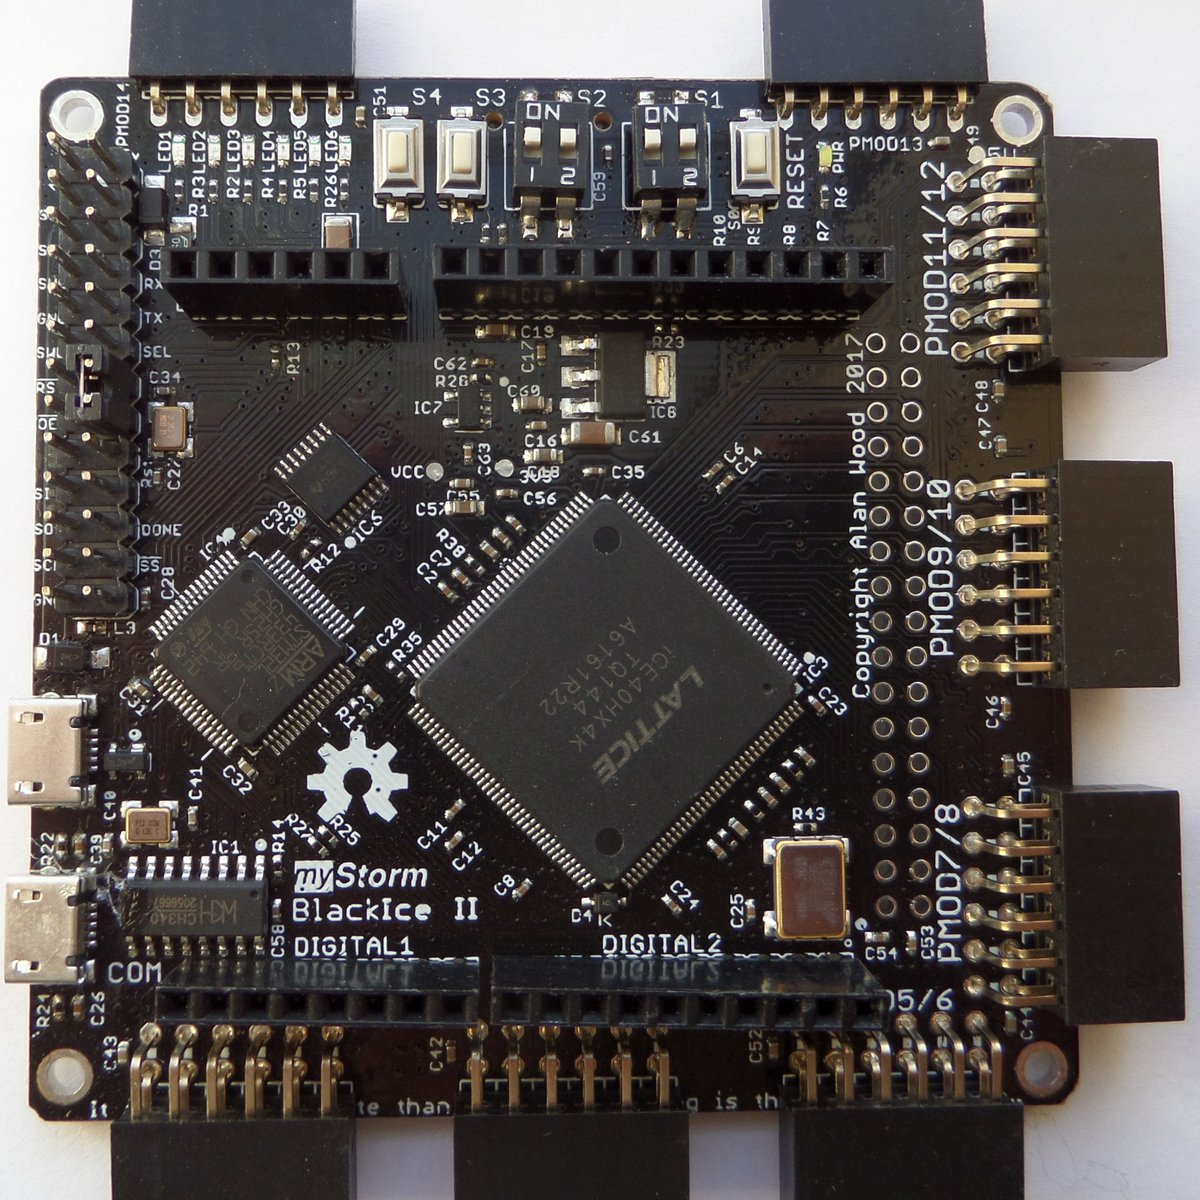
\includegraphics[trim = 0mm 0mm 0mm 0mm, clip,scale=0.2]{imagenes/EstadoArte/BlackIce.jpg}
		\caption{BlackIce II}
		\label{fig:blackIceII}
	\end{figure}
\end{center}
\begin{center}
	\begin{figure}[H]
		\center
		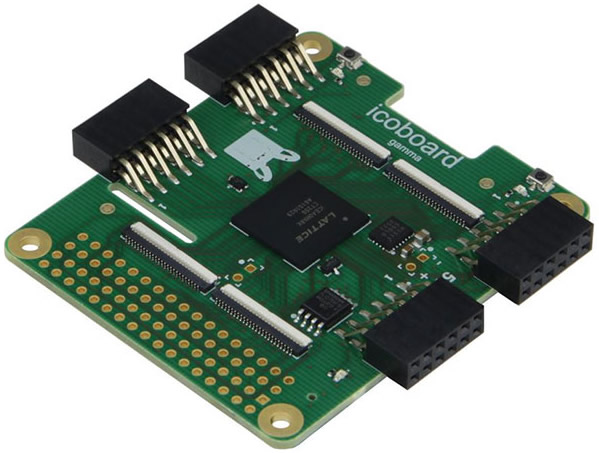
\includegraphics[trim = 0mm 0mm 0mm 0mm, clip,scale=0.4]{imagenes/EstadoArte/ico_board.jpg}
		\caption{ico Board}
		\label{fig:icoBoard}
	\end{figure}
\end{center}
\subsection{IceZum Alhambra}
Para este trabajo se ha optado por trabajar con la IceZum Alhambra, la cuál ha sido íntegramente diseñada y ensamblada en España.\newline
Es una FPGA libre y compatible con IceStudio (el cuál se analizará en a sección \ref{sec:IceStudio}). Alguna de sus características más importantes son:
\begin{itemize}
	\item Placa FPGA de desarrollo iCE40HX1K-TQ144 de la empresa Lattice. 
	\item Open hardware.
	\item Compatible con IceStorm toolchain.
	\item Compatible con shields de Arduino Uno. 
	\item 12MHz Oscilador.
	\item Interuptor ON/OFF para activar o desactivar los pines digitales.
	\item 20 Input/output 5v pines.
	\item 8 Input/Output 3.3V pines
	\item USB micro-B para programar la FPGA desde el pc.
	\item Botón de reset.
	\item 8 leds de proposito general.
	\item TX/RX Leds
	\item 4 entradas analógicas disponibles a través de i2c.
\end{itemize}

Es conocido que existen placas con mejores carácterísticas, pero el hecho de que sea Open Hardware y que se pueda implementar con IceStudio, ha llevado a la elección final de esta tarjeta para el desarrollo del presente proyecto.\newline
\begin{center}
\begin{figure}[H]
	\center
	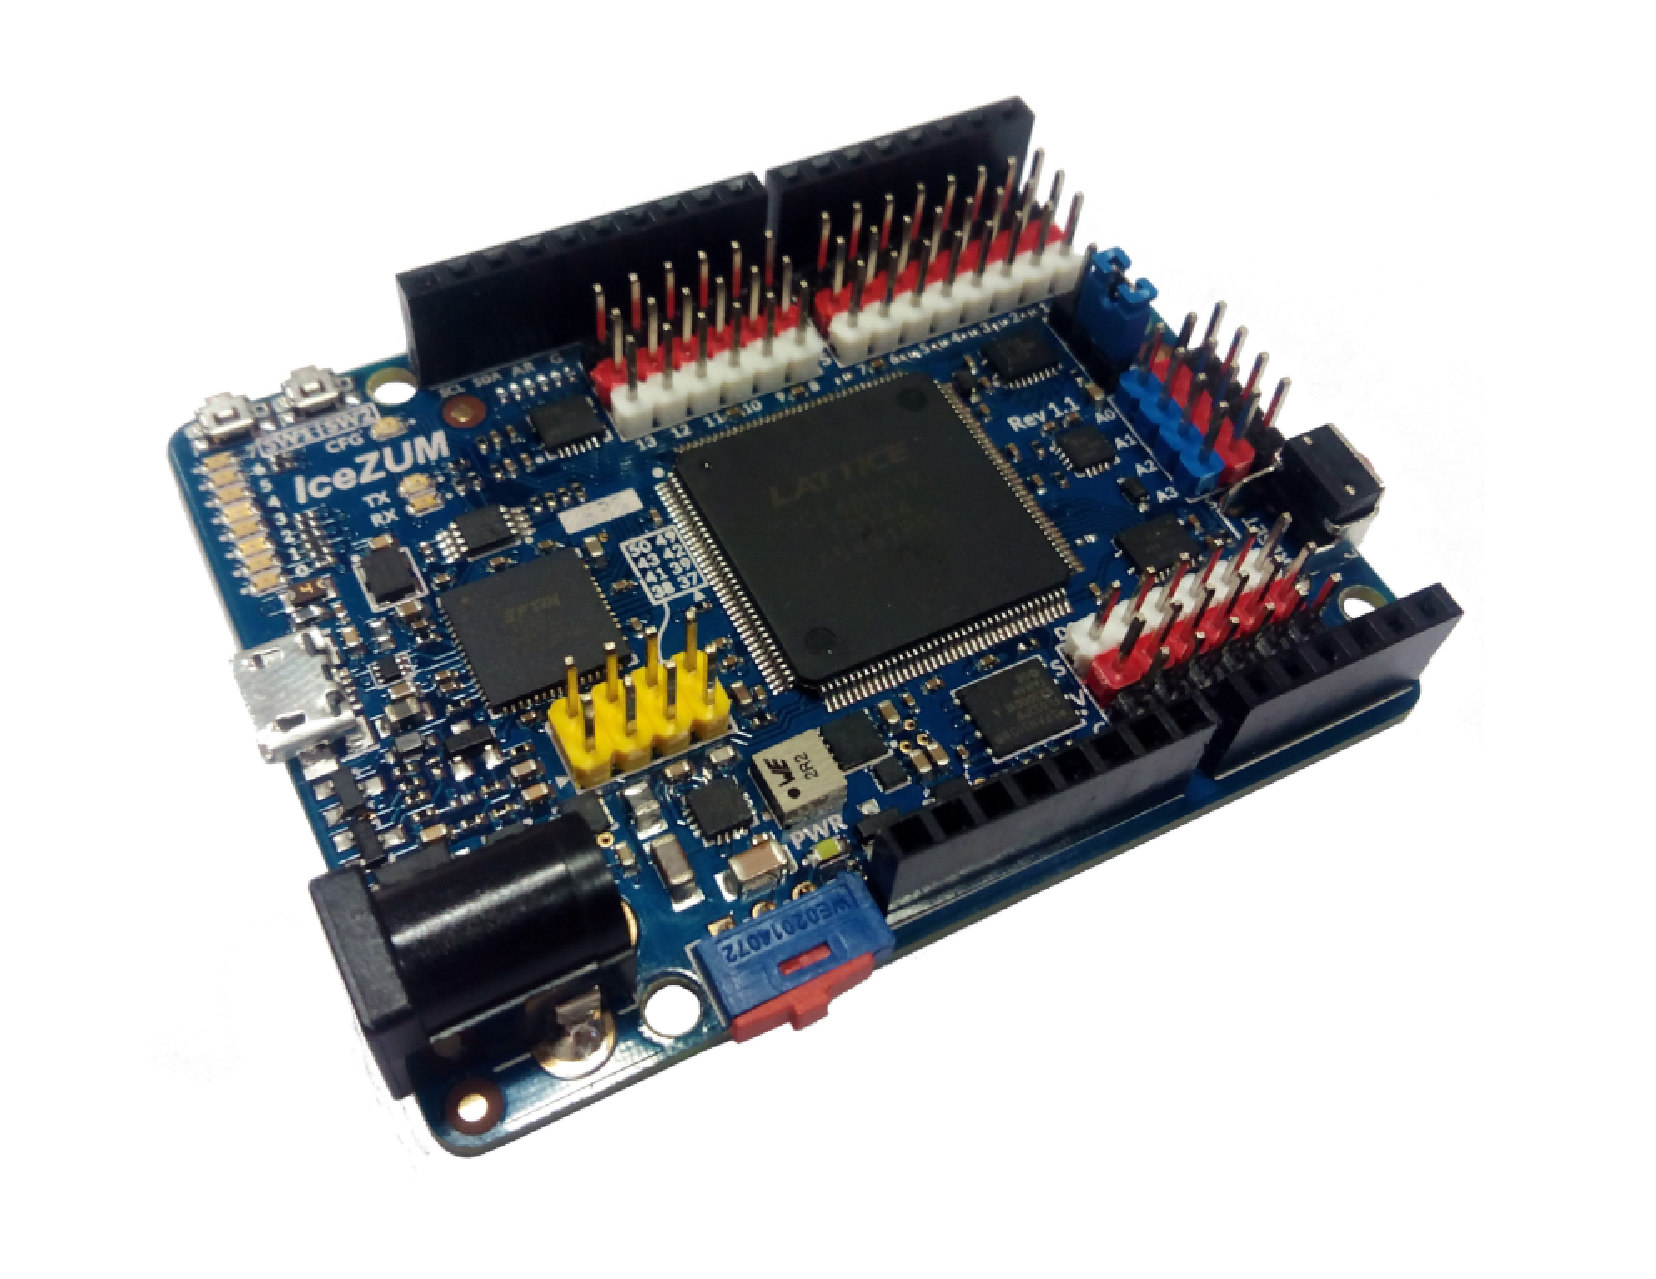
\includegraphics[scale=0.4]{imagenes/EstadoArte/IceZumAlhambra.pdf}
	\caption{IceZum Alhambra Board}
	\label{fig:IceZumAlhambraI}
\end{figure} 
\end{center}
Un punto a tener en cuenta para el desarrollo hardware con esta FPGA es su memoria de 1K lo que ha supuesto una limitación importante en el desarrollo. Para el presente proyecto se ha hecho uso también de la nueva versión de la IceZum Alhambra, IceZum Alhambra II, la cuál aún no estaba en el mercado al inicio del proyecto y que conlleva algunas mejoras, como la ampliación de 8K en su memoria, la mejora del bus de datos i2c, la posibilidad de alimentación mediante batería LIPO, etc. \newline
La IceZum Alhambra se representa en la figura \ref{fig: IceZumAlhambraII}
\begin{center}
	\begin{figure}[H]
		\center
		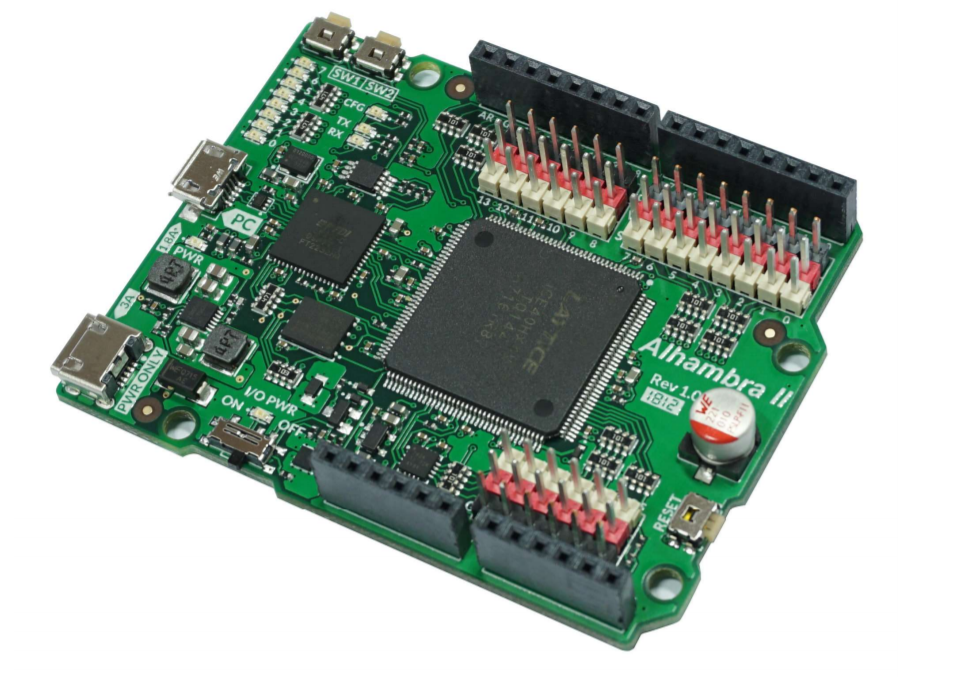
\includegraphics[scale=0.5]{imagenes/EstadoArte/IceZumAlhambra.PNG}
		\caption{IceZum Alhambra II Board}
		\label{fig: IceZumAlhambraII}
	\end{figure} 
\end{center}


\subsection{IceStudio}\label{sec:IceStudio}
Los lenguajes HDL suelen tener una curva de aprendizaje difícil, debido esto en gran medida al nivel de abstracción tan bajo necesario para diseñar un sistema en concreto. Es necesario conocer las características hardware de nuestro sistema para poder trabajar con este tipo de lógica. \newline

Como se ha desarrollado anteriormente, algunos fabricantes proporcionan herramientas comerciales para programar sus propias FPGA. Si bien en la actualidad son entornos complejos, cuentan con una gran cantidad de herramientas y funcionalidades. Lamentablemente la mayoría de ellos no son gratuitos y están unidos a la arquitectura de un único fabricante.
\newline
Con la evolución de las FPGAs han empezado a aparecer lenguajes que permiten un mayor nivel de abstracción. 
Además, también han aparecido herramientas centradas en la implementación gráfica. Un ejemplo de este tipo de implementación es LabVIEW FPGA o IceStudio. \newline
IceStudio es un proyecto Open Source desarrollado por Jesús Arroyo Torrens y en el que nos basaremos a lo largo del presente documento. \newline

IceStudio es IDE gráfico para FPGAs libres y esta construido sobre el proyecto IceStorm. 
El proyecto IceStorm tiene como objetivo la ingenieria inversa y la documentación del formato bitstream de la FPGA Lattice iCE40 (aunque más adelante fueron surgiendo algunas más). Proporciona herramientas simples para analizar y crear archivos de flujo de bits, esto es, el más bajo de nivel de implementación para una FPGA.\newline

Para acercar al lector al conocimiento y funcionamiento de IceStudio se irán incorporando a lo largo del documento una serie de capturas de pantalla representativas para que no se pierda la visión de lo que se esta haciendo. Por ejemplo, la ventana principal de IceStudio y sobre la que se desarrollará todo lo demás tendrá la apariencia que se muestra en la \ref{fig:Main_IceStudio}: \newline

\begin{figure}[H]
	\center
	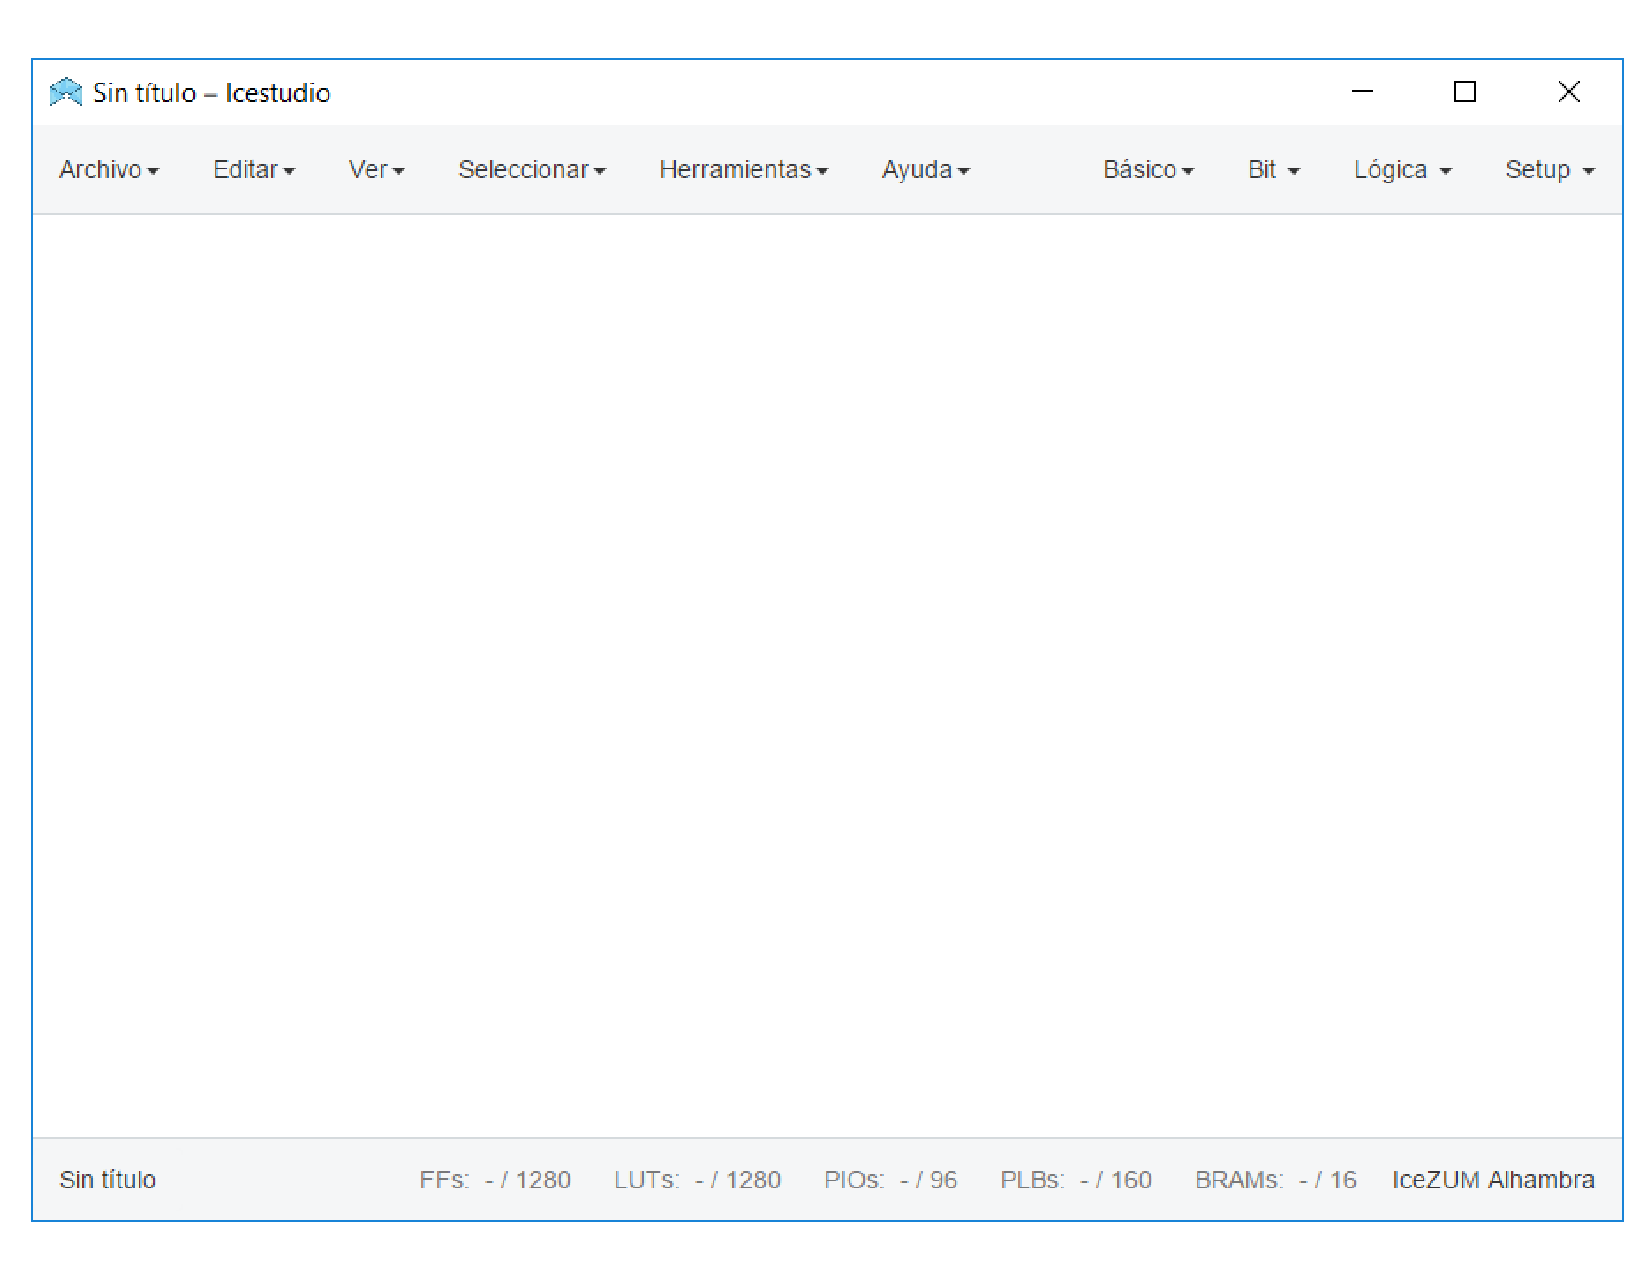
\includegraphics[trim = 0mm 20mm 0mm 0mm, clip,scale=0.6]{imagenes/EstadoArte/Main_IceStudio.pdf}
	\caption{Ventana principal IceStudio.}
	\label{fig:Main_IceStudio}
\end{figure}

El hecho de que IceStudio sea un editor gráfico puede hacer pensar que el nivel de abstracción podría ser más alto de lo deseado, pero lo cierto es que este nivel es configurable. \newline
Es el usuario final el que decide con que nivel de abstracción se trabaja, siendo necesario para eso una amplia biblioteca de módulos como veremos a continuación. Para poder explicar la potencia de IceStudio, se procederá con un caso práctico;\newline

El módulo que se presenta en la figura \ref{fig:Write_i2c_module} es una escritura normal de i2c, en la cuál se parametriza la dirección del esclavo y la dirección que se quiere leer (más adelante se explicará con más detalle). \newline

\begin{figure}[H]
	\center
	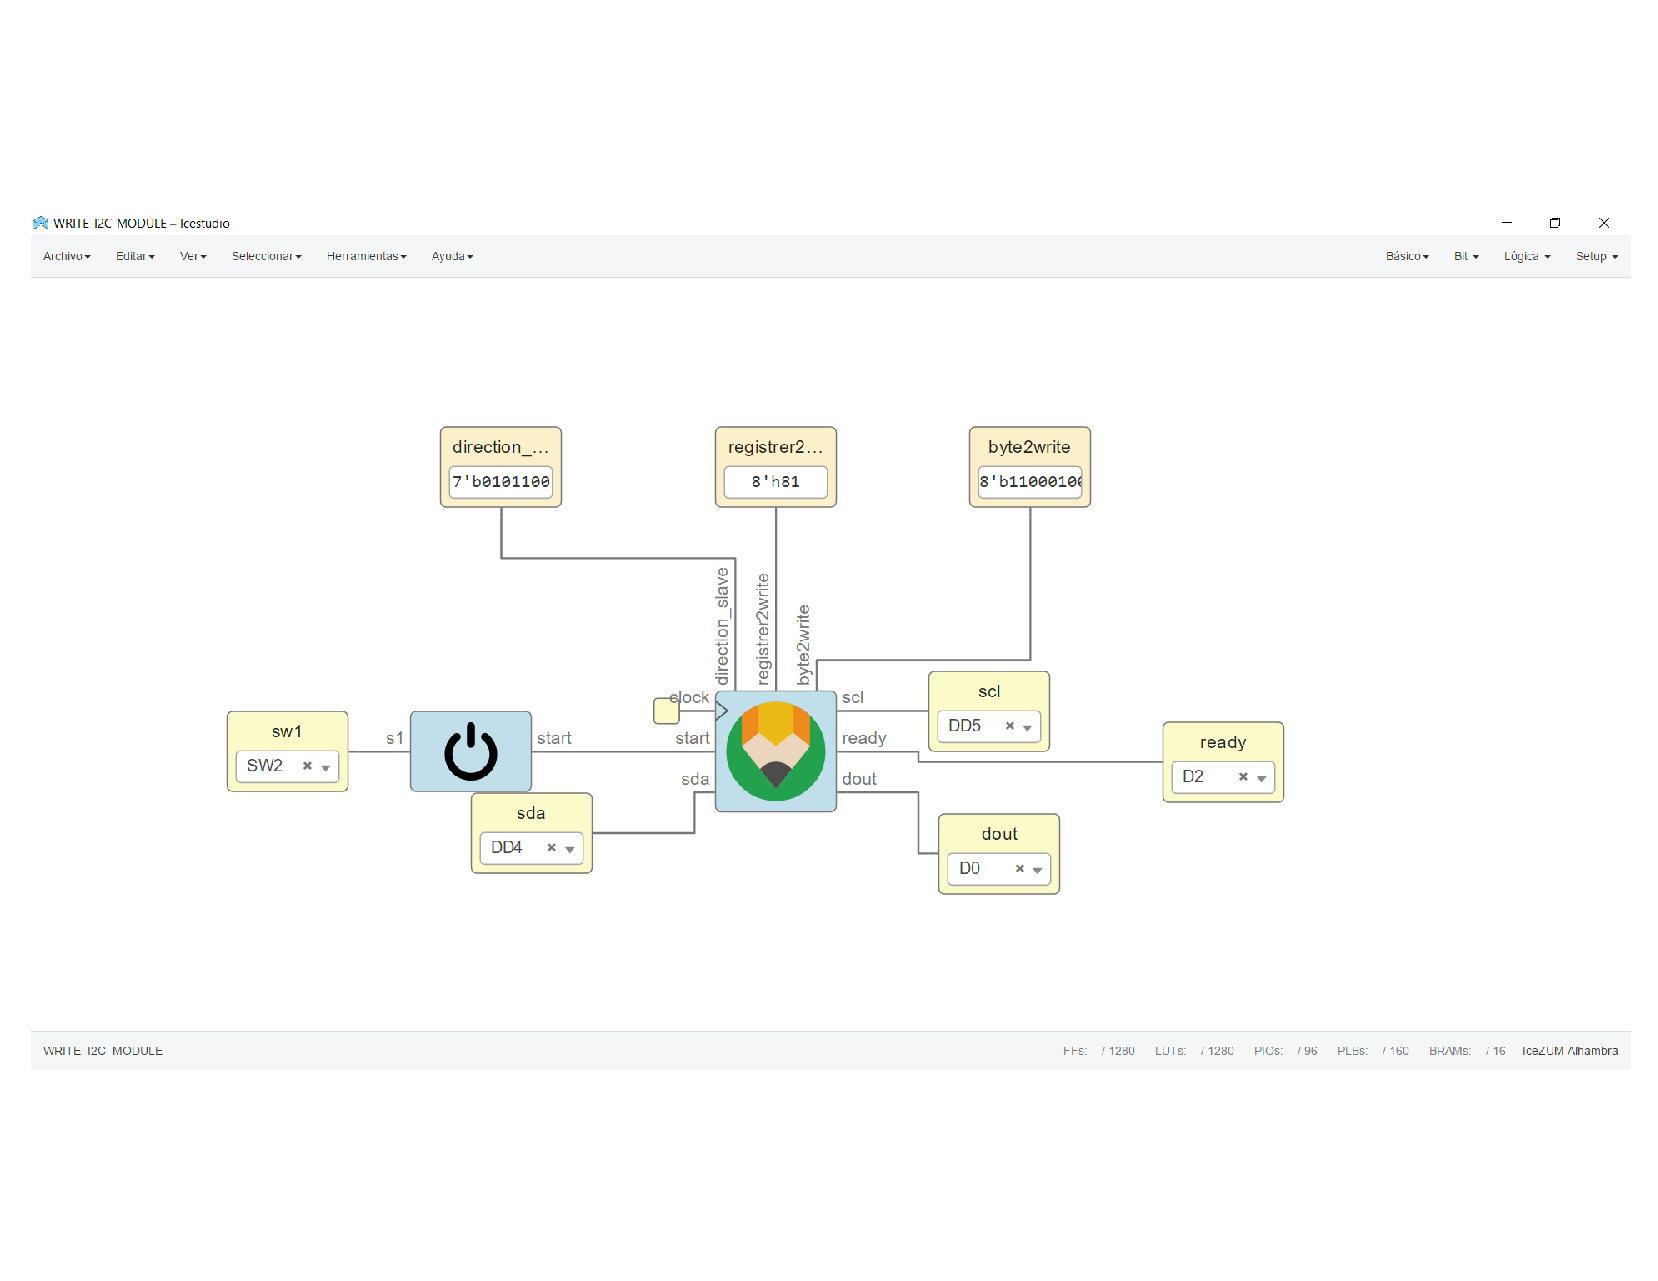
\includegraphics[trim = 0mm 25mm 0mm 0mm, clip,scale=0.6]{imagenes/EstadoArte/Write_i2c_module.pdf}
	\caption{Escritura I2C IceStudio alto nivel.}
	\label{fig:Write_i2c_module}
\end{figure}

Así, si una persona no experimentada con este tipo de código y cuyo fin no es entenderlo quiere hacer uso de eso no deberá de bajar mucho de nivel.\newline
No obstante, existe la posibilidad de que se requieran cambiar valores como la frecuencia de reloj, el modo de operación i2c, etc.
Para ello podemos bajar de nivel e introducirnos en el módulo en cuestión, en este caso, haciendo doble clic, como aparece en la figura \ref{fig:Write_i2c_module2}. 

\begin{figure}[H]
	\center
	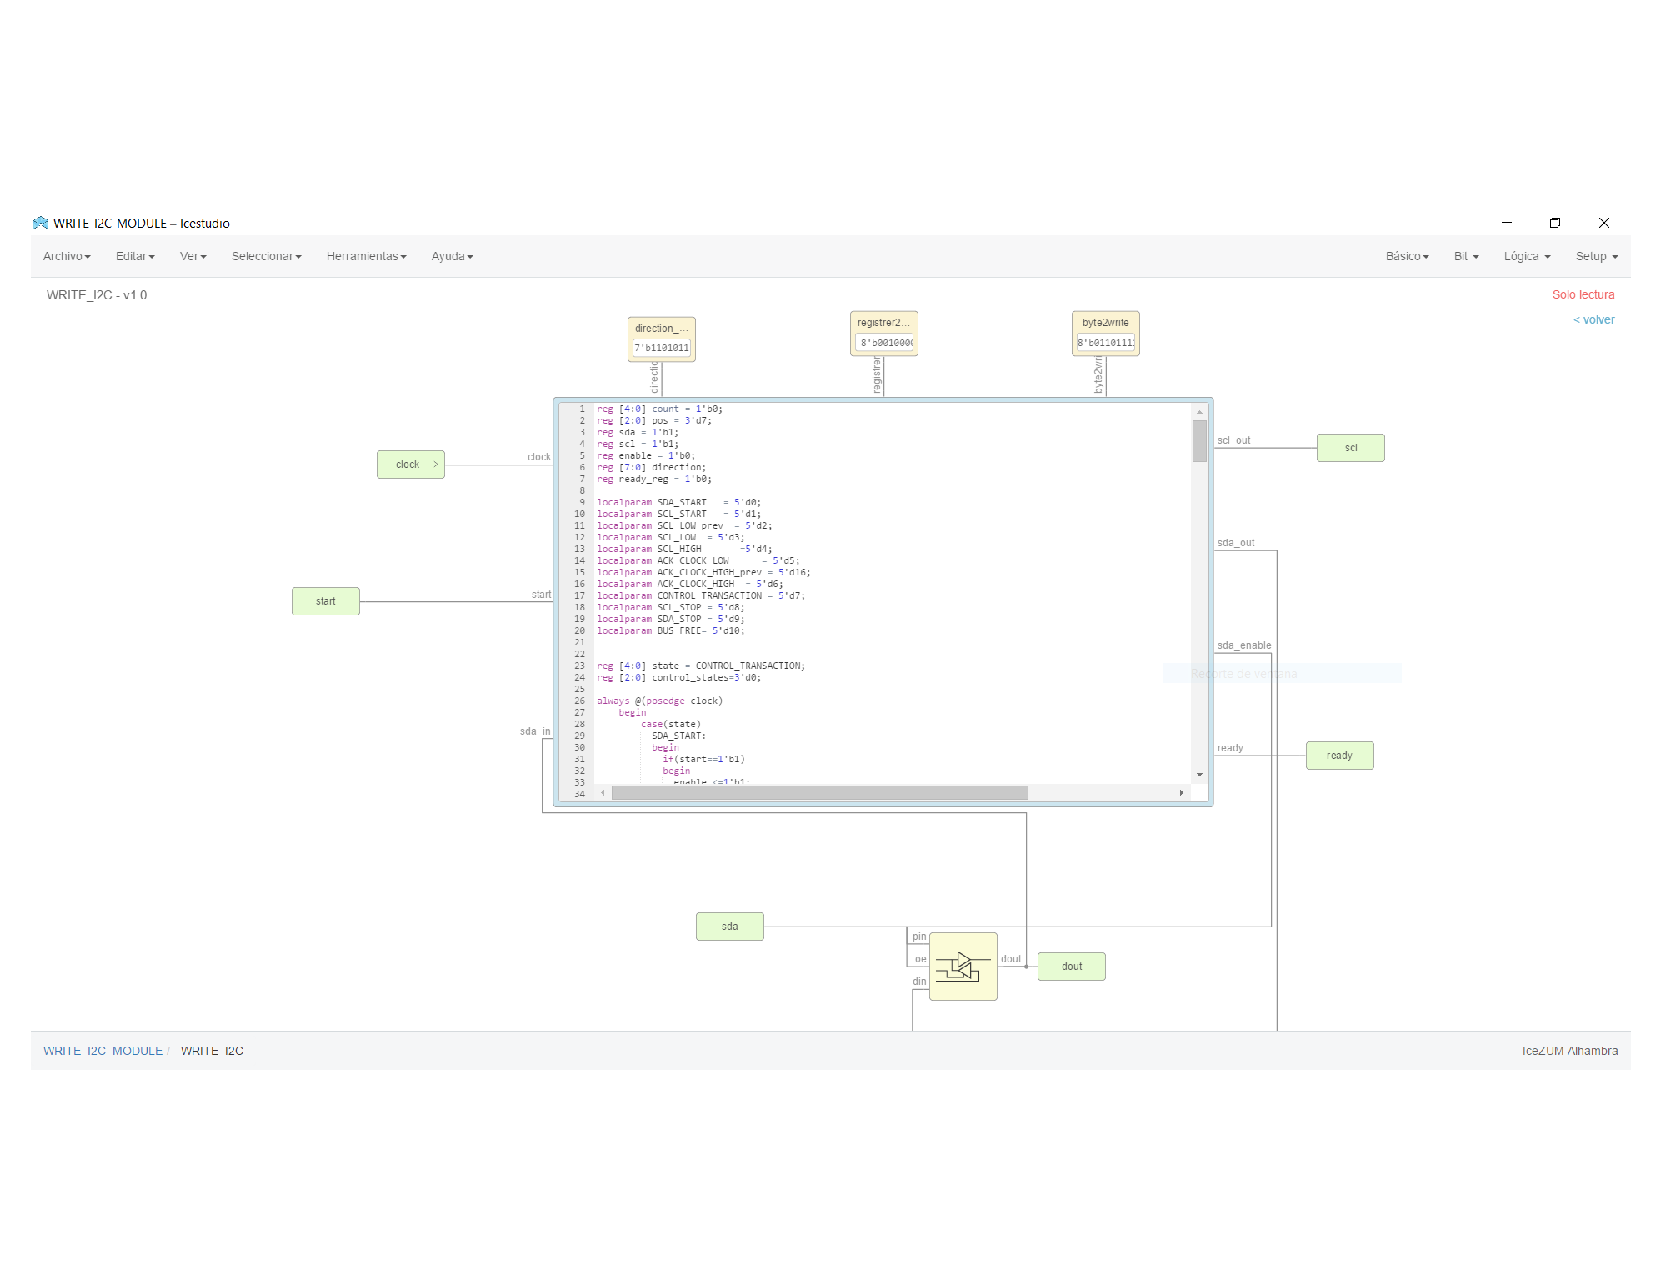
\includegraphics[trim = 0mm 20mm 0mm 0mm, clip,scale=0.6]{imagenes/EstadoArte/Write_i2c_module2.pdf}
	\caption{Escritura I2C IceStudio bajo nivel.}
	\label{fig:Write_i2c_module2}
\end{figure}

Se podría decir entonces que se ha bajado un nivel más de abstracción, pudiendo entrar ahora en detalles hardware más específicos si fuese necesario. \newline

En la anterior caso práctico se ha podido ver una de las ventajas de IceStudio. La modularidad permite configurar el nivel de abstracción.
Para ello hace falta una biblioteca de módulos, algunos de los cuáles serán desarrollados a lo largo de este trabajo, otros de ellos, están siendo desarrollados, y pueden encontrarse en el siguiente enlace: 

\href{https://groups.google.com/forum/#!topic/fpga-wars-explorando-el-lado-libre/I3ZnqKlfh5M}{Foro de Google con discusión sobre temas y módulos para IceStudio.}


%%%%%%%%%%%%%%%%%%%%%%%%%%%%%%%%%%%%%%%%%%%%%%%%%
\section{Coexistencia Microcontrolador-FPGA}\label{sec:coexistencia}
\subsection{Diferencia microcontrolador-FPGA}
En un principio puede parecer que un procesador y FPGA son dispositivos similares porque ambos pueden realizar ciertas tareas pre-configuradas. Lo cierto es que al profundizar se pueden encontrar mas diferencias que similitudes. Ambos son capaces de implementar una función de transferencia, pero la forma en la que lo hacen es diferente para cada uno de ellos.\newline

Así, podríamos ver las FPGA y los microcontroladores como una caja negra en la que tenemos unas entradas y ciertas salidas tal y como se muestra en la figura \ref{fig:funcionalidad_FPGA_micro}.\newline


\begin{figure}[H]
	\center
	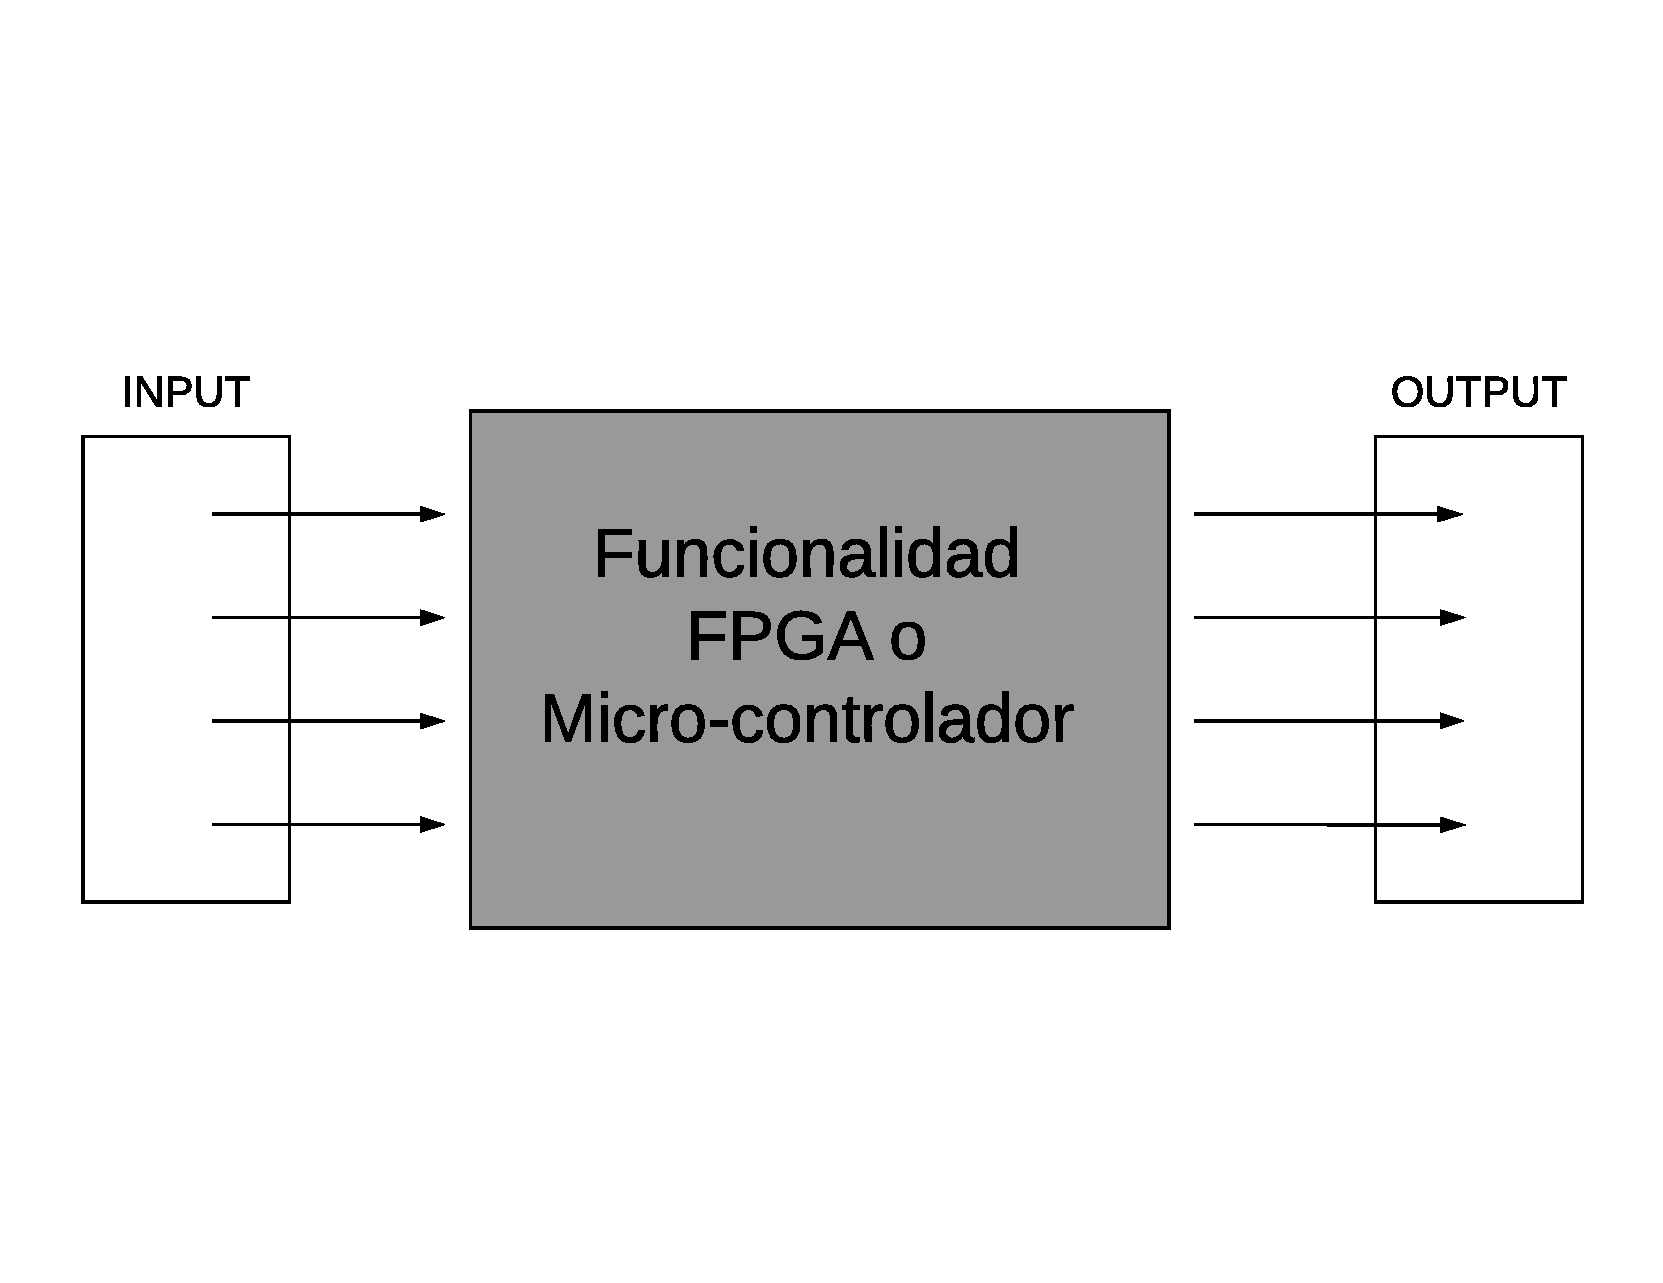
\includegraphics[trim = 0mm 30mm 0mm 30mm, clip,scale=0.4]{imagenes/EstadoArte/funcionalidad_FPGA_micro.pdf}
	\caption{Funcionalidad FPGA y Micro-controlador.}
	\label{fig:funcionalidad_FPGA_micro}
\end{figure}

Para comprobar de forma resumida como implementan de manera diferente esa función de transferencia, se explicará brevemente la forma de trabajar con un procesador. \newline
Un procesador contiene una serie de instrucciones que realizan operaciones sobre un conjunto de bits (sumar, incrementar, leer y escribir de la memoria). Dependiendo del tipo de procesador y de su arquitectura tenemos más o menos instrucciones asociadas, siendo este aspecto uno de los mas importantes que determinan su rendimiento.

\textbf{Arquitectura procesador}

Se dispone de una serie de registros, una memoria para almacenar la información y una pila de instrucciones, que contiene el programa que va a ejecutarse en código máquina, además de un reloj.\newline

Su modo de funcionamiento a alto nivel; en cada ciclo de reloj el procesador lee de su pila de instrucciones los valores necesarios, llama a la instrucción oportuna y ejecuta un determinando cálculo.\newline
Como se argumentó en la sección \ref{sec:ArquitecturaFPGA}, al implementar un diseño lógico en una FPGA, se está modificando una matriz de conexiones físicas. Modificando esa matriz de conexiones se pueden implementar diferentes bloques de funcionalidad, es decir, se podría representar como varias funciones de transferencia en un mismo sistema hardware.\newline
En la figura \ref{fig:puertas_logicas} se representa un ejemplo real de como están implementadas las conexiones físicas de puertas lógicas en una FPGA, y de como eso permite tener módulos independientes unos de otros. Además, notese el problema de la memoria en una FPGA, siendo está el número total de puertas lógicas físicas que pueden ser utilizadas.
\begin{center}
\begin{figure}[H]
	\center
	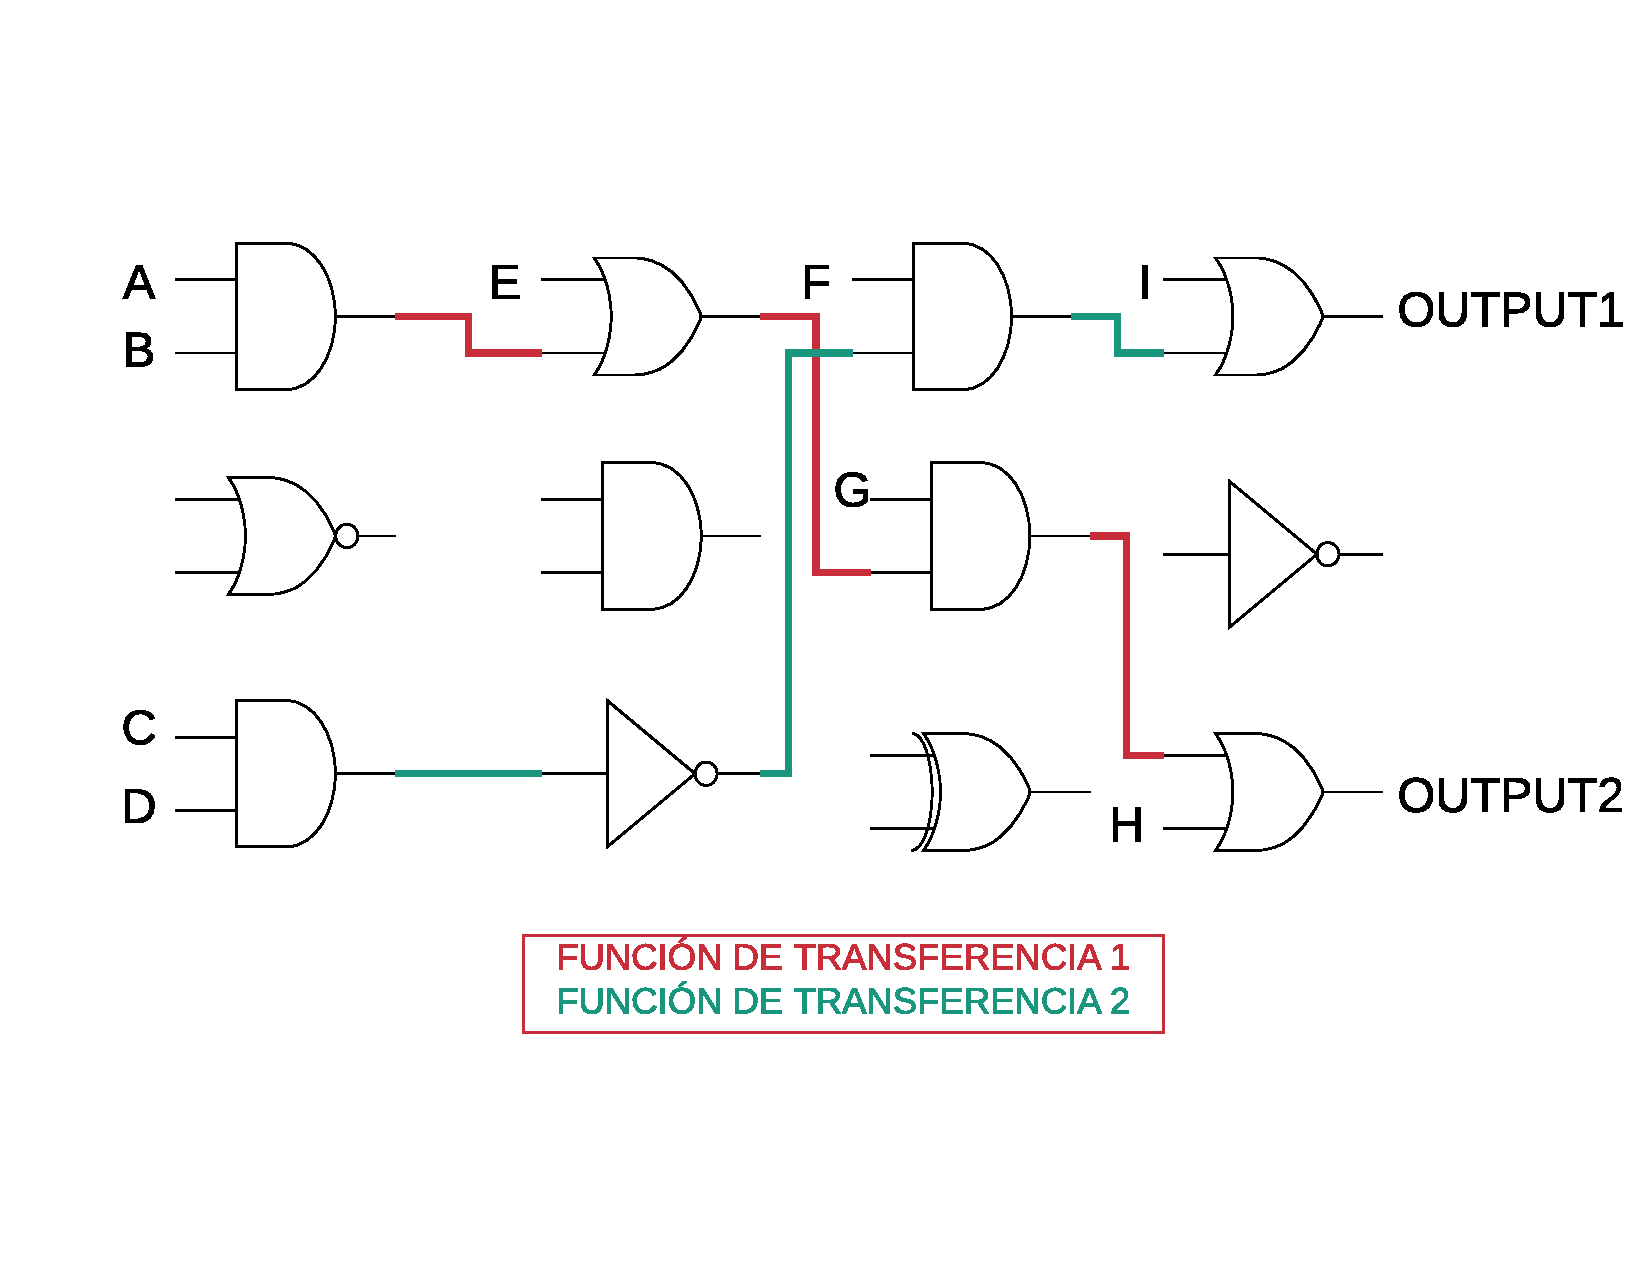
\includegraphics[scale=0.4]{imagenes/EstadoArte/puertas_logicas.pdf}
	\caption{Puertas lógicas después de una implementación hardware.}
	\label{fig:puertas_logicas}
\end{figure}
\end{center} 

\subsection{Necesidad}

Se imagina un ejemplo real el que se quieren monitorizar con exactitud 4 diferentes sensores provenientes del exterior, de una manera exacta, al mismo tiempo y a la velocidad del reloj, siendo necesaria además una posterior actuación por parte del sistema. El diagrama de bloques del flujo de trabajo en un procesador que implemente lo anterior podría parecerse al siguiente:

\tikzstyle{block_circle} = [draw, fill=blue!20, circle, 
minimum height=3em, minimum width=6em]
\tikzstyle{block_rectangle} = [draw, fill=blue!20, rectangle, 
minimum height=3em, minimum width=6em]
%\tikzstyle{sum} = [draw, fill=blue!20, circle, node distance=1cm]
\tikzstyle{input} = [coordinate]
\tikzstyle{output} = [coordinate]
%\tikzstyle{pinstyle} = [pin edge={to-,thin,black}]

% The block diagram code is probably more verbose than necessary
\begin{center}
\begin{tikzpicture}[auto, node distance=2cm,>=latex']
	% We start by placing the blocks
	\node [input, name=input] {};
	\node [block_circle, right of=input] (Sensor1) {Sensor1};
	\node [block_rectangle, right of= Sensor1, node distance=3cm] (actuador1) {actuador1};
	\node [block_circle, right of=actuador1,node distance=3cm] (Sensor2) {Sensor2};
	\node [block_rectangle, right of= Sensor2, node distance=3cm] (actuador2) {actuador2};
	\node [block_circle, below of=actuador2,node distance=3cm] (Sensor3) {Sensor3};
	\node [block_rectangle, left of= Sensor3, node distance=3cm] (actuador3) {actuador3};
	\node [block_circle, left of=actuador3,node distance=3cm] (Sensor4) {Sensor4};
	\node [block_rectangle, left of= Sensor4, node distance=3cm] (actuador4) {actuador4};
	
	
	% We draw an edge between the controller and system block to 
	% calculate the coordinate u. We need it to place the measurement block. 
	
	% Once the nodes are placed, connecting them is easy. 
	\draw [draw,->] (Sensor1) -- node {} (actuador1);
	\draw [draw,->] (actuador1) -- node {} (Sensor2);
	\draw [draw,->] (Sensor2) -- node {} (actuador2);
	\draw [draw,->] (actuador2) -- node {} (Sensor3);
	\draw [draw,->] (Sensor3) -- node {} (actuador3);
	\draw [draw,->] (actuador3) -- node {} (Sensor4);
	\draw [draw,->] (Sensor4) -- node {} (actuador4);   
	
	
	
	
\end{tikzpicture}
\end{center}

Así, el usuario final de este sistema, deberá de manera cíclica comprobar cada sensor y su posterior actuación, dejando de cumplir entonces las especificaciones de tiempo. \newline
Si se trabajase con interrupciones se configurarían las diferentes interrupciones externas o se podrían usar ejecutivos cíclicos para acercarse a esos requerimientos finales. No obstante, cualquiera de estas soluciones, no dejan de ser una aproximación.\newline

En cambio, con el uso de una FPGA, el diagrama de bloques del flujo de trabajo tendría el siguiente aspecto:

\tikzstyle{block} = [draw, fill=blue!20, rectangle, 
minimum height=3em, minimum width=6em]
%\tikzstyle{sum} = [draw, fill=blue!20, circle, node distance=1cm]
\tikzstyle{input} = [coordinate]
\tikzstyle{output} = [coordinate]
%\tikzstyle{pinstyle} = [pin edge={to-,thin,black}]
\begin{center}

% The block diagram code is probably more verbose than necessary
\begin{tikzpicture}[auto, node distance=4cm,>=latex']
% We start by placing the blocks
\node [block] (sensor1) {Sensor1};
\node [block, right of=input] (function1) {$F_{1}$};
\node [block, right of= function1, node distance=4cm] (actuar) {actuadores};


% We draw an edge between the controller and system block to 
% calculate the coordinate u. We need it to place the measurement block. 

% Once the nodes are placed, connecting them is easy. 
\draw [draw,->] (sensor1) -- node {$$} (function1);
\draw [draw,->] (function1) -- node {$$} (actuar);



\end{tikzpicture}
\end{center}

\begin{center}
\begin{tikzpicture}[auto, node distance=4cm,>=latex']
% We start by placing the blocks
\node [block] (sensor2) {Sensor2};
\node [block, right of=input] (function2) {$F_{2}$};
\node [block, right of= function2, node distance=4cm] (actuar) {actuadores};


% We draw an edge between the controller and system block to 
% calculate the coordinate u. We need it to place the measurement block. 

% Once the nodes are placed, connecting them is easy. 
\draw [draw,->] (sensor2) -- node {$$} (function2);
\draw [draw,->] (function2) -- node {$$} (actuar);



\end{tikzpicture}
\end{center}

\begin{center}
\begin{tikzpicture}[auto, node distance=4cm,>=latex']
% We start by placing the blocks
\node [block] (sensor3) {Sensor3};
\node [block, right of=input] (function3) {$F_{3}$};
\node [block, right of= function3, node distance=4cm] (actuar) {actuadores};


% We draw an edge between the controller and system block to 
% calculate the coordinate u. We need it to place the measurement block. 

% Once the nodes are placed, connecting them is easy. 
\draw [draw,->] (sensor3) -- node {$$} (function3);
\draw [draw,->] (function3) -- node {$$} (actuar);



\end{tikzpicture}
\end{center}

\begin{center}
\begin{tikzpicture}[auto, node distance=4cm,>=latex']
% We start by placing the blocks
\node [block] (sensor4) {Sensor4};
\node [block, right of=input] (function4) {$F_{4}$};
\node [block, right of= function1, node distance=4cm] (actuar) {actuadores};


% We draw an edge between the controller and system block to 
% calculate the coordinate u. We need it to place the measurement block. 

% Once the nodes are placed, connecting them is easy. 
\draw [draw,->] (sensor4) -- node {$$} (function4);
\draw [draw,->] (function4) -- node {$$} (actuar);



\end{tikzpicture}
\end{center}



Se implementarían diferentes funciones de transferencia para cada uno de los bloques a desarrollar, pudiendo ejecutarse estos en paralelo. \newline

No obstante, no siempre es necesario un ejecutivo en paralelo, y no solo puede no ser necesario sino que podría ser perjudicial. Cuando un sistema debe ser secuencial, ¿porqué utilizar una implementación de naturaleza paralela?. \newline

Es muy común tener sistemas donde conviene poder implementar ambos tipos de funcionamiento, por eso una coexistencia FPGA/Micro-controlador podría ser suficiente para adaptarse a los requerimientos. \newline

En la imagen \ref{fig:bipedo} se puede ver como ejemplo real de un sistema bípedo, el cuál se explicará con mas detalle en los siguientes capítulos:

\begin{center}
	\begin{figure}[H]
		\center
		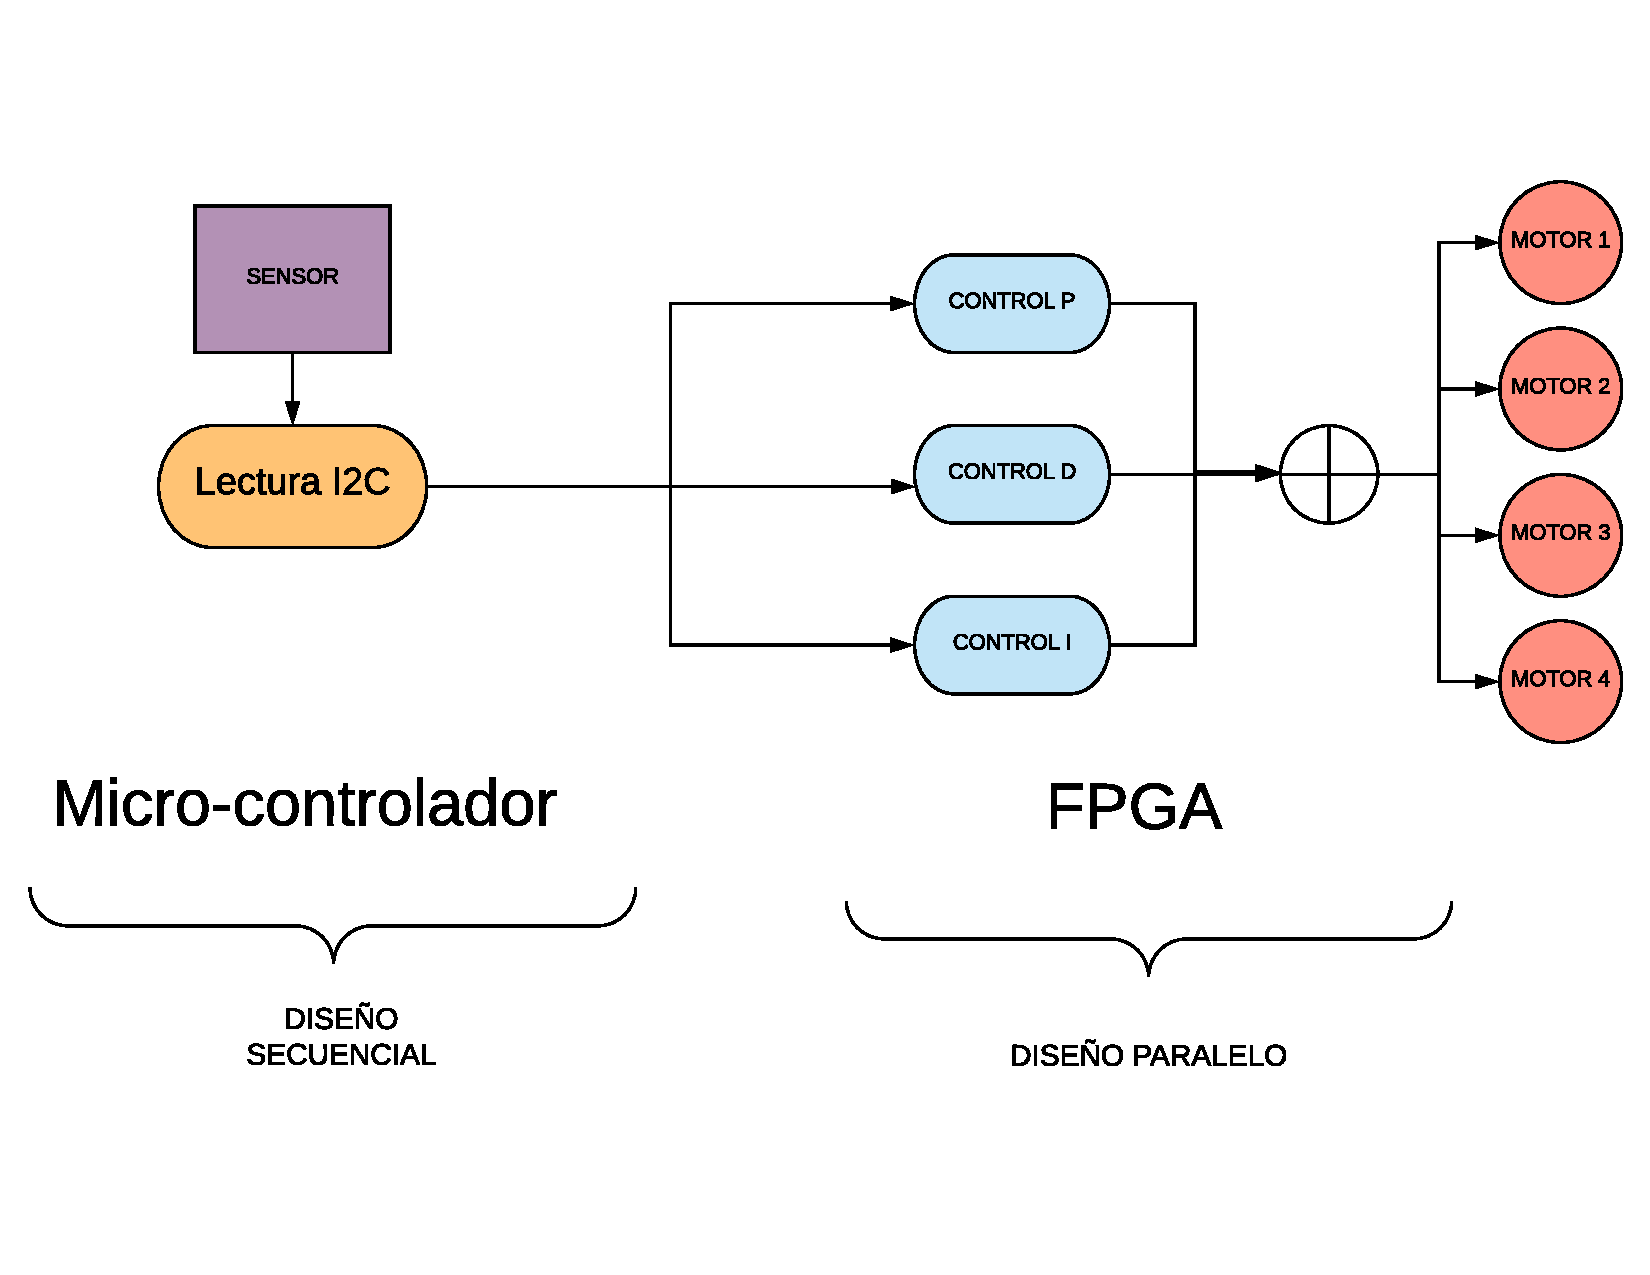
\includegraphics[scale=0.5]{imagenes/EstadoArte/bipedo.pdf}
		\caption{Sistema bipedo coexistencia Micro-FPGA.}
		\label{fig:bipedo}
	\end{figure}
\end{center}
%%%%%%%%%%%%%%%%%%%%%%%%%%%%%%%%%%%%%%%%%%%%%%%%%
\section{Unidad de medida inercial}
El componente central del sistema propuesto esta definido como IMU o unidad de medida inercial. Está compuesto por una serie de sensores los cuales serán utilizados para conocer de manera exacta aspectos de localización del sistema a bordo tales como velocidad, orientación, fuerzas gravitacionales etc. \newline
Esta información puede ser utilizada para el control o el simple conocimiento del sistema en un momento concreto. \newline

En el caso del presente proyecto, será utilizado para obtener los ángulos de navegación o ángulos de Tait-Brain, en los que la orientación se presenta con tres rotaciones ortogonales en torno al eje X, Y y Z. Un ejemplo de este tipo de representación se encuentra en la figura \ref{fig:orientacion}\newline


\begin{figure}[H]
	\center
	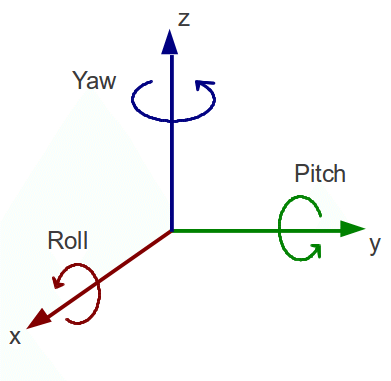
\includegraphics[scale=0.5]{imagenes/Balancing_robot/orientacion}
	\caption{Ángulos de Tait-Brain.}
	\label{fig:orientacion}
\end{figure}


Una IMU queda definida por su número de grados de libertad (DOF) los cuáles dependerán del número de sensores a bordo (acelerómetro, giroscopio) y el número de ejes en los que se aplican. Así una IMU con seis grados de libertad (por ejemplo un acelerómetro de 3 ejes y un giroscopio de 3 ejes) se diría que es 6DOF. \newline

En las figuras \ref{fig:IMU1}, \ref{fig:IMU2}, \ref{fig:IMU2} se presentan algunos ejemplos de IMUs.

\begin{figure}[H]
	\center
	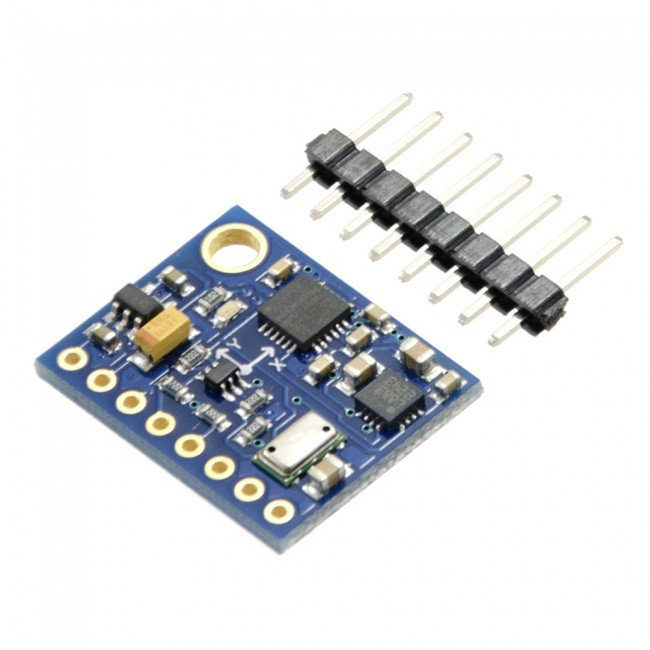
\includegraphics[scale=0.2]{imagenes/Balancing_robot/IMU1}
	\caption{Unidad de Medida Inercial.}
	\label{fig:IMU1}
\end{figure}

\begin{figure}[H]
	\center
	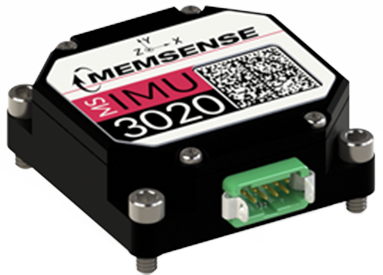
\includegraphics[scale=0.2]{imagenes/Balancing_robot/IMU2}
	\caption{Unidad de Medida Inercial.}
	\label{fig:IMU2}
\end{figure}

\begin{figure}[H]
	\center
	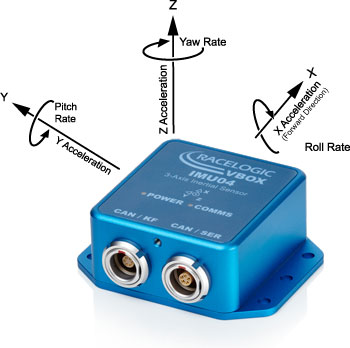
\includegraphics[scale=0.2]{imagenes/Balancing_robot/IMU3}
	\caption{Unidad de Medida Inercial.}
	\label{fig:IMU3}
\end{figure}

Otra de las características importantes y de la cuál dependerá en gran medida el precio del producto es el rango de los sensores a bordo y de la disponibilidad en el propio sistema de conversores analógico digitales, encargados estos de convertir el valor del sensor a un valor binario que pueda ser utilizado para posterior análisis. \newline
A continuación se definen algunos de los aspectos más importantes que pueden ser encontrados en una unidad de medida inercial y los cuáles serán muy útiles a lo largo del presente proyecto.

\subsubsection{Acelerómetro}
Un acelerómetro, como su propio nombre indica es un dispositivo que permite medir la aceleración a la que un cuerpo está sometido. Es un componente fundamental en las unidades de medida inercial pues se puede detectar por ejemplo, condiciones de caída libre, aunque el principal uso es para determinar la orientación del sensor. \newline

Los acelerómetros normalmente son de tres ejes, es decir, son capaces de medir independientemente la aceleración en el eje X, Y y Z, lo que permite conocer la magnitud y dirección del vector aceleración en cada uno de los ejes. \newline

El caso que interesa en este proyecto es poder determinar la orientación del sensor. Para ello, se debe aplicar tigonometría. Suponiendo un sistema 2D con el representado en la figura \ref{fig:acelerometro1}.

\begin{figure}[H]
	\center
	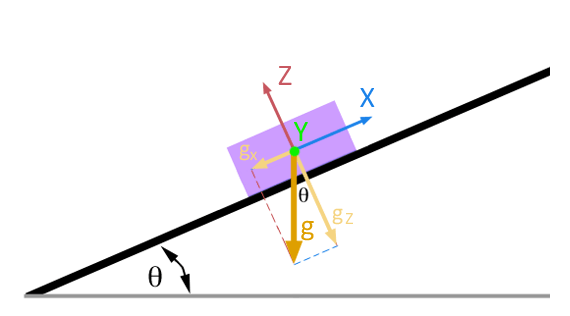
\includegraphics[scale=0.4]{imagenes/Balancing_robot/acelerometro1}
	\caption{Trigonométrica en sensor acelerómetro 2D.}
	\label{fig:acelerometro1}
\end{figure}

\begin{equation}
\theta = atan\frac{A_{x}}{A_{z}}
\end{equation}

Si se aplica en una representación 3D como la representada en la \ref{fig:acelerometro2}

\begin{figure}[H]
	\center
	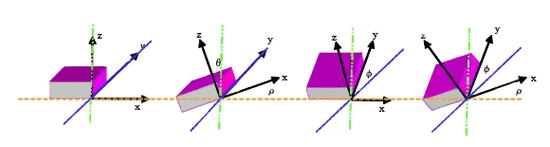
\includegraphics[scale=0.6]{imagenes/Balancing_robot/acelerometro2}
	\caption{Trigonométrica en sensor acelerómetro 3D.}
	\label{fig:acelerometro2}
\end{figure}

\begin{equation}
\theta_{x} = atan\frac{A_{x}}{\sqrt{A_{y^2}+A_{z^2}}}
\end{equation}

\begin{equation}
\theta_{y} = atan\frac{A_{y}}{\sqrt{A_{x^2}+A_{z^2}}}
\end{equation}

\begin{equation}
\theta_{z} = atan\frac{A_{z}}{\sqrt{A_{x^2}+A_{y^2}}}
\end{equation}

\subsubsection{Giroscopio}
Un giroscopio es un dispositivo que permite medir el ángulo de rotación de un determinado dispositivo. \newline

En un giroscopio, siempre se miden ángulos relativos a una referencia arbitraria (a diferencia de los acelerómetros). El giroscopio que se emplea en ente proyecto es denominado giroscopio vibratorio de efecto Coriolis. \newline

Al igual que en el acelerometro del apartado anterior, los giroscopios suelen emplear tres ejes, es decir, son capaces de registrar de forma independiente la rotación en los ejes X, Y y Z, se tiene por tanto el modulo y dirección del vector de rotación. \newline

Es importante tener en cuenta que este tipo de giroscopios basados en el efecto Coriolis no detectan el ángulo girado sino la velocidad angular, aspecto importante para su depuración. \newline

Si se recuerda el concepto de velocidad angular (ecuación \ref{equation:velangular});

\begin{equation} \label{equation:velangular}
\omega = \frac{\delta \omega}{\delta t}
\end{equation}

Así, para obtener el ángulo es necesario realizar la integración respecto del tiempo (ecuación \ref{equation:integracion}).

\begin{equation}\label{equation:integracion}
\theta_{gyro} = \omega_{gyro}*\Delta t
\end{equation}

Los acelerómetros son dispositivos que frecuentemente son muy sensibles a las vibraciones, por lo que para su correcto procesamiento hay que tener en cuenta que presentará mucho ruido de alta frecuencia. Un filtrado a una frecuencia determinada resolverá parte de este problema.\newline

Tener que hacer una integración con respecto al tiempo lleva consigo algunos problemas, los cuáles serán vistos en la siguiente sección. 

\subsubsection{Problema de deriva}

Gran parte de las unidades de medida inercial del mercado están compuestas como mínimo de acelerómetros y giroscopios, el motivo de esta combinación es que uno complementa las limitaciones del otro y viceversa. \newline

La deriva en un sensor electrónico o "drift" es una variación con el tiempo de la salida del medidor (con respecto a la medida real) a pesar de que la variable pueda ser constante, es provocado en cierta medida por cambios en la temperatura o por la acumulación de errores. \newline

Tanto en un acelerómetro con en un giroscopio encontramos errores asociados a la deriva: 
\begin{itemize}
	\item Los acelerómetros no tienen deriva a medio o largo plazo, sin embargo, se ven influenciados por los movimientos del sensor y el ruido por lo que no son fiables a medio o corto plazo.
	\item En cuanto a los giroscopios, funcionan muy bien en movimientos bruscos y cortos pero al realizar una integración con respecto al tiempo aparece el problema de deriva a medio o largo plazo. 
\end{itemize} 

Después de analizar los problemas de ambos, parece razonable poder combinar ambas mediciones para obtener orientaciones más precisas. 

\subsubsection{Posibles soluciones}

Para solucionar algunos de los problemas anteriores, puede ser muy útil aplicar algunas de las soluciones propuestas a contunuación: 

\begin{itemize}
	\item Combinar y filtrar las señales mediante un filtro complementario. Es el más utilizado en la actualidad debido a su no muy elevada complejidad. Su expresión más sencilla se representa en la ecuación \ref{equation:complementary_filter}.
	\begin{equation} \label{equation:complementary_filter}
	\theta = A * (\theta_{prev}+\theta_{gyro}) + B * \theta_{accel}
	\end{equation}
	\item Combinar y filtrar las señales mediante un filtro de Kalman, el cuál realiza una estimación del valor futuro de la medición. Sin embargo, utiliza unos cálculos complejos. 
	\item Algunas unidades de medida inercial incorporan de manera interna procesadores DMPs (Digital Motion Processor) los cuáles ejecutan complejos algoritmos evitando tener que realizar filtros y liberando al sistema de procesamiento.
\end{itemize}



Una vez explicados las características básicas de las IMUs comerciales, en la sección \ref{sec:MPU6050} se desarrollará la IMU elegida para este sistema y sus carácterísticas propias.

\subsection{Controlador de motores}
Tener un modulo con la capacidad para generar PWM soluciona muchos problemas posteriores a la vez que mejora la visibilidad del código en el sistema final. Como se observa en las características de los motores, gran parte de ellos están comandados por una señal PWM que si bien es cierto, depende del motor en cuestión. \newline
La modulación por ancho de pulsos o PWM (Pulse Width Modulation) es una técnica en la que se modifica el ciclo de trabajo de una señal periódica (en nuestro caso cuadrada) que se usa para transmitir información a traves de un canal de comunicación o para controlar la cantidad de energía que se envía a una carga. Un ejemplo de una señal PWM cuadrada es la mostrada en la figura tal 

\textbf{figura PWM}

Aplicando esta señal, por ejemplo, a un motor DC clásico se varia la cantidad de energía que se aplica a la carga, el motor en este caso. Sencillamente funciona como un interruptor en el cuál un nivel lógico alto es abierto y un nivel bajo cerrado. Si se consigue variar el tiempo el cuál al motor le esta llegando carga y el tiempo en el cuál no le llega corriente, se puede controlar su velocidad. \newline

Así, las características de una señal PWM son: 
\begin{itemize}
	\item D = ciclo de trabajo.
	\item $\theta$
	\item T = periodo de la función
\end{itemize}

\section{PID clásico}
\section{Robótica educativa, motivaciones y necesidad.}

La robótica se puede considerar sin duda como una de las áreas tecnológicas con mas auge de la actualidad y basada en el estudio de los robots, que son sistemas compuestos por mecanismos que le permiten hacer movimientos y realizar tareas específicas, programables e inteligentes. \newline

Dependiendo de la aplicación por tanto, la robótica puede extenderse y generar beneficios no sólo en la industria sino también en las aulas de clase, posibilitando la aparición de nuevos sistemas de aprendizaje.\newline

Además en un mundo cuyo futuro va encaminado a la utilización de robots para cualquier actividad, el acercamiento desde las aulas con estos sistemas posibilita su desarrollo tecnológico a una edad temprana, siendo más fácil su integración a una edad adulta.\newline

Algunos beneficios de la robótica educativa son expuestos a continuación:  
\begin{itemize}
	\item Impulsa la iniciativa y la creatividad
	\item Mayor sociabilización
	\item Incentiva el pensamiento algorítmico y matemático
	\item Trabajo en equipo
	\item Resolución de problemas
	\item Aprendizaje activo
	\item Aumento de la autoestima
\end{itemize}

No obstante, para que la integración en las aulas de la robótica educativa sea aún mas fácil, los sistemas deben cumplir algunas características:

\begin{itemize}
	\item No es recomendable la integración a alto nivel tecnológico.
	\item Los robots deben ser de carácter amigable y divertido. 
	\item Los entornos de programación no deben ser complejos, y aunque su funcionalidad este algo limitada, tiene que llamar la atención del alumno y hacerle sentir cómodo.
	\item Es importante que el robot cuente con una serie de sensores y actuadores, unas entradas y salidas para que los resultados sean visuales.
\end{itemize}

Después de haber analizado cuáles son las ventajas de la electrónica digital, resulta conveniente poder acercar estos dos campos de conocimiento; electrónica digital-robótica educativa.\newline

Si la electrónica digital y el mundo de los robots están llamados a formar parte de nuestras vidas en un futuro cercano, la necesidad de un acercamiento a estos dos conceptos a edades tempranas es básico para un correcto avance de la tecnología. \newline

Con esta idea nace IceStudio, hacer amigable la electrónica digital para que los más pequeños puedan hacer uso de ella, y además, cumple todas las características antes expuestas.

\section{Sensores, actuadores y sistema de control }

Antes de comenzar con el desarrollo del proyecto, es importante tener claro los conceptos de sensores, actuadores y elementos del sistema de control, los cuáles forman parte de cualquier plataforma robótica móvil. \newline

Cualquier instalación de control, ya sea robótica o inmótica, esta compuesta por tres componentes fundamentales:
\begin{itemize}
	\item Sensores
	\item Actuadores
	\item Sistema de control
\end{itemize}

Los sensores son dispositivos que recogen información del mundo que nos rodea y lo transforma en señales eléctricas que puedan ser asimiladas por un sistema de control. \newline

Así, el sistema de control recibe información del entorno sobre el que queremos realizar algún tipo de acción por medio de los sensores, es la función de transferencia del sistema, a partir de unas entradas de tipo conocido, son generadas unas salidas, normalmente, dependientes de las entradas. \newline

Estas salidas son denominadas actuadores, que son dispositivos que, siguiendo los parámetros dados por el sistema de control realizan acciones que repercuten en el entorno. \newline

\textsl{Ejemplo: Un sensor indica al sistema de control la intensidad lumínica de nuestra habitación, el sistema de control reconoce que el nivel no es el adecuado para la lectura, y activa un actuador, en este caso, una luz, para contrarrestar ese nivel.}

A la hora de elegir un determinado sensor, es importante conocer su modo de operación, para poder configurar o mantener sistemas que los incorporen. Existen diferentes tipos de sensores según:

\begin{itemize}
	\item Tipo de salida: \begin{itemize}
		\item Analogicos
		\item Binarios
		\item Digitales
	\end{itemize} 
	
	\item Estructura interna: \begin{itemize}
		\item Pasivos
		\item Activos
	\end{itemize}
	
	\item Tipo de parámetros capaces de detectar
\end{itemize}
 En tabla \ref{tabla:modo_operacion_sensores} se muestran algunos de los más interesantes para el desarrollo del proyecto:

\renewcommand\tablename{Tabla}
\begin{table}[H]
	\begin{center}
	\begin{tabular}{|c|l|l|}
		\hline
		\textbf{Magnitud}                                                                       & \multicolumn{1}{c|}{\textbf{Transductor}} & \multicolumn{1}{c|}{\textbf{Característica}} \\ \hline
		\multirow{2}{*}{\begin{tabular}[c]{@{}c@{}}Posición lineal y\\   angular\end{tabular}}  & Potenciómetro                             & Analógica                                    \\ \cline{2-3} 
		& Encoder                                   & Digital                                      \\ \cline{2-3} 
		& Sensor Hall                               & Digital                                      \\ \hline
		\multirow{2}{*}{\begin{tabular}[c]{@{}c@{}}Velocidad\\   lineal y angular\end{tabular}} & Dinamo tacométrica                        & Analógica                                    \\ \cline{2-3} 
		& Encoder                                   & Digital                                      \\ \cline{2-3} 
		& Detector inductivo                        & Digital                                      \\ \cline{2-3} 
		& Servo-inclinómetros                       & A/D                                          \\ \cline{2-3} 
		& RVDT                                      & Analógica                                    \\ \cline{2-3} 
		& Giróscopo                                 & Digital                                      \\ \hline
		\multirow{2}{*}{Aceleración}                                                            & Acelerómetro                              & Analógico                                    \\ \cline{2-3} 
		& Servo-accelerómetros                      &                                              \\ \hline
		\multirow{2}{*}{Visión artificial}                                                      & Cámaras de video                          & Procesamiento digital                        \\ \cline{2-3} 
		& Cámaras CCD o CMOS                        & Procesamiento digital                        \\ \hline
	\end{tabular}
	\caption{Modo de operación de sensores.}
	\label{tabla:modo_operacion_sensores}
\end{center}
\end{table}

Otra clasificación posible es la del ámbito de aplicación, es decir, donde y para qué son usados estos sensores. \newline
De entre las carácterísticas técnicas más importantes de un sensor, y haciendo una introducción al posible vocabulario que se utilizará, encontramos:

\begin{itemize}
	\item Rango de medida:  dominio en la magnitud medida en el que puede aplicarse el sensor.
	\item Precisión: es el error de medida máximo esperado.
	\item Offset o desviación de cero: valor de la variable de salida cuando la variable de entrada es nula.
	\item Sensibilidad de un sensor: suponiendo que es de entrada a salida y la variación de la magnitud de entrada.
	\item Resolución: mínima variación de la magnitud de entrada que puede detectarse a la salida.
	\item Derivas: son otras magnitudes, aparte de la medida como magnitud de entrada, que influyen en la variable de salida.
\end{itemize}

Por lo general, la señal de salida de estos sensores no es apta para su lectura directa y a veces tampoco para su procesado, por lo que se usan circuitos de acondicionamiento. Un ejemplo de algunos sensores se representan en las figuras \ref{fig:camara_CMOS}, \ref{fig:IMU} y \ref{fig:potentiometer}.

\begin{center}
	\begin{figure}[H]
		\center
		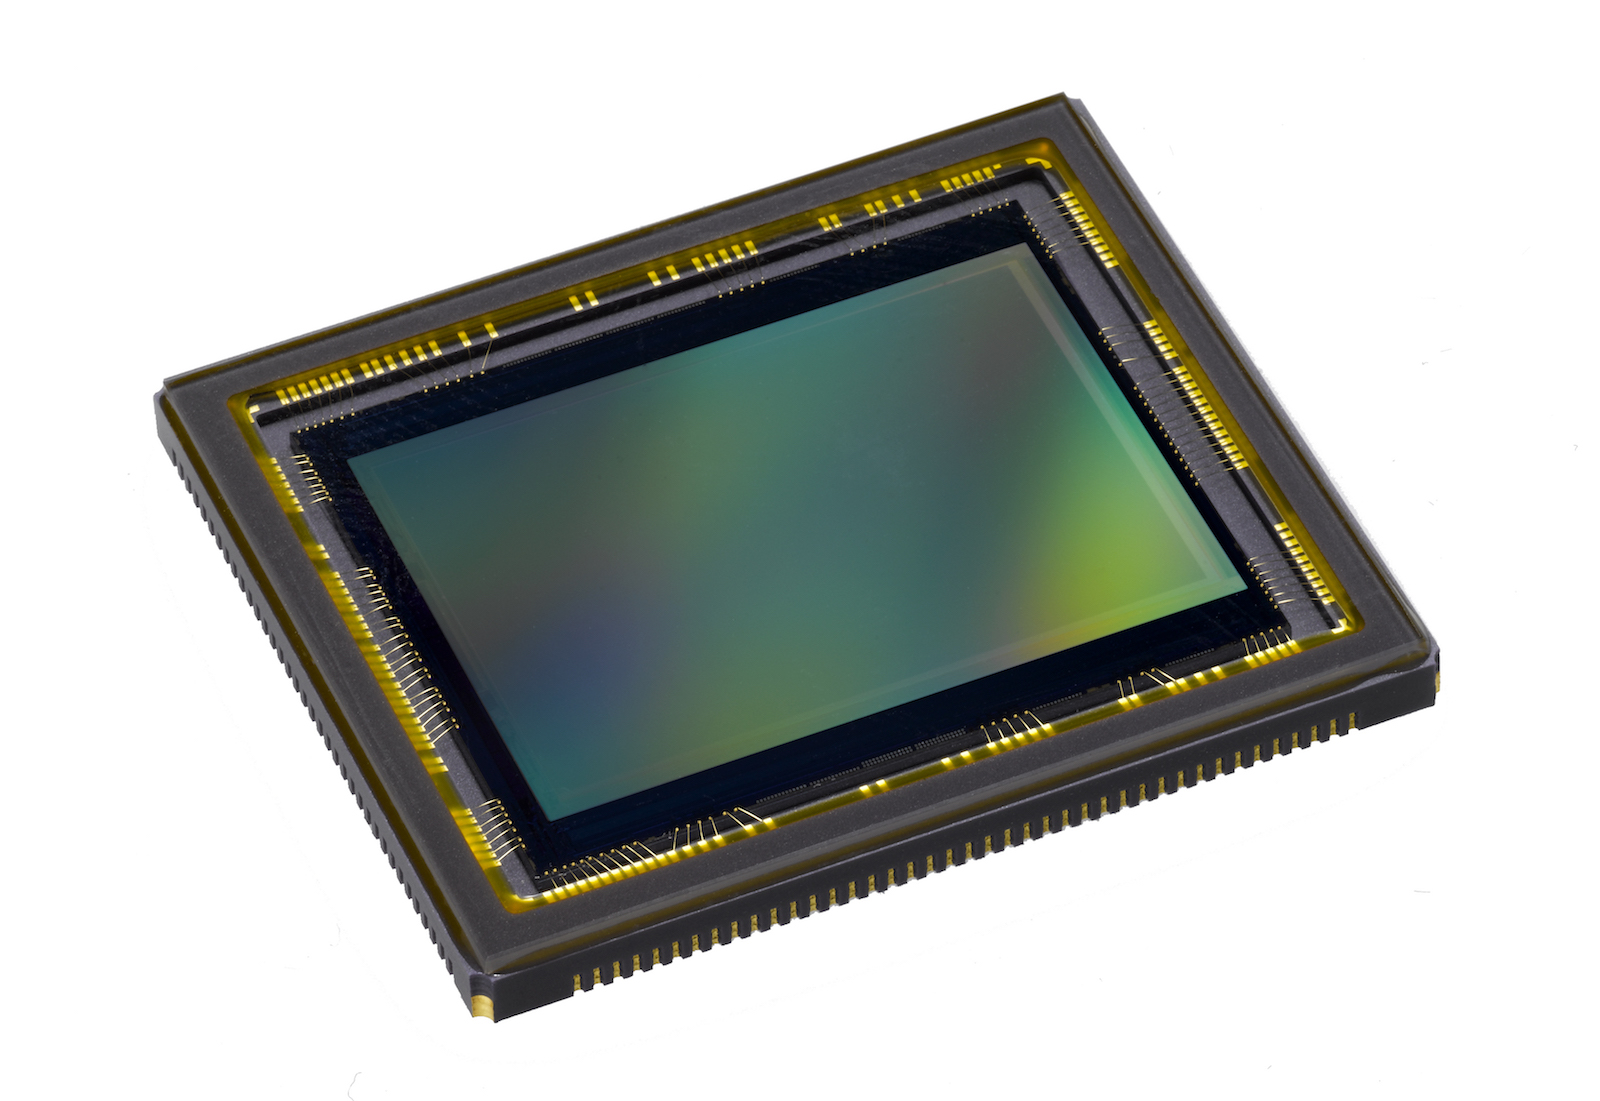
\includegraphics[scale=0.1]{imagenes/EstadoArte/sensor_imagen_CMOS.jpg}
		\caption{Sensor CMOS para adquisición de imágenes.}
		\label{fig:camara_CMOS}
	\end{figure}
\end{center}

\begin{center}
	\begin{figure}[H]
		\center
		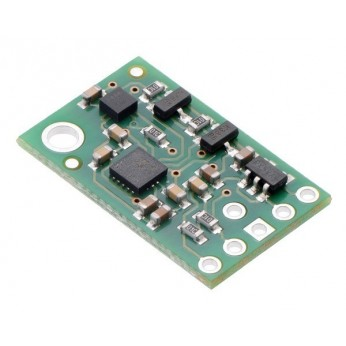
\includegraphics[scale=0.4]{imagenes/EstadoArte/IMU.jpg}
		\caption{Unidad de Medida Inercial.}
		\label{fig:IMU}
	\end{figure}
\end{center}

\begin{center}
	\begin{figure}[H]
		\center
		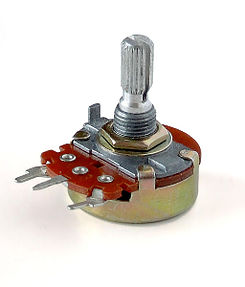
\includegraphics[scale=0.4]{imagenes/EstadoArte/potentiometer.jpg}
		\caption{Potenciómetro.}
		\label{fig:potentiometer}
	\end{figure}
\end{center}

Los actuadores son dispositivos que permiten al sistema de control ‘actuar’ sobre el ‘mundo real’ para realizar las acciones deseadas. Uno de los actuadores mas conocidos son los motores, el cuál será muy utilizado a lo largo de esta aplicación.  \newline

\begin{center}
	\begin{figure}[H]
		\center
		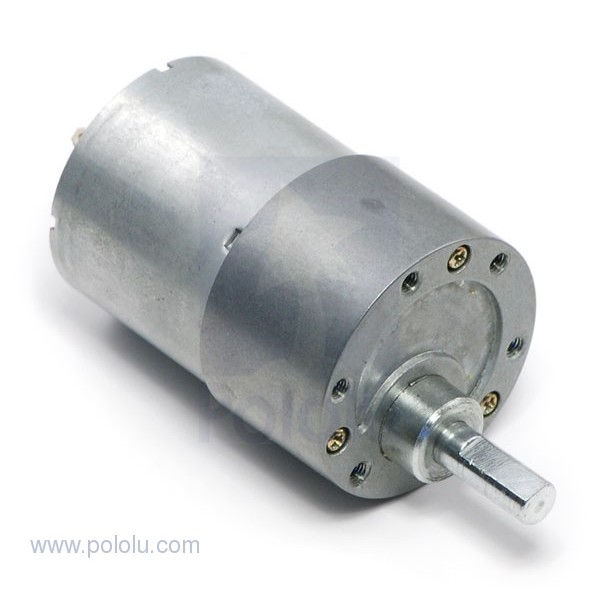
\includegraphics[scale=0.4]{imagenes/EstadoArte/motor.jpg}
		\caption{Motor DC.}
		\label{fig:motor_DC}
	\end{figure}
\end{center}


Sistemas de control hay de muchos tipos en relación de la aplicación la cual se quiere desarrollar, normalmente se elije un micro-controlador como sistema de control y se programa la función de transferencia a ser realizada.\newline
En el caso de este proyecto, y para poder adquirir por un lado las ventajas de una FPGA y por otro las ventajas de un micro-controlador (seccion \ref{sec:coexistencia}), se utilizará tanto arduino para las tareas secuenciales como la IceZum Alhambra para las tareas que puedan ser paralelizadas. \newline


